\documentclass[a4paper, 10pt, twoside]{article}

\usepackage[top=1in, bottom=1in, left=1in, right=1in]{geometry}
\usepackage[utf8]{inputenc}
\usepackage[spanish, es-ucroman, es-noquoting]{babel}
\usepackage{setspace}
\usepackage{fancyhdr}
\usepackage{lastpage}
\usepackage{amsmath}
\usepackage{amsfonts}
\usepackage{amsthm}
\usepackage{verbatim}
\usepackage{graphicx}
\usepackage{float}
\usepackage[noend]{algpseudocode}
\usepackage{enumitem} % Provee macro \setlist
\usepackage[toc, page]{appendix}
\usepackage{amsthm}
\usepackage{epstopdf}
\usepackage{amssymb}
\usepackage{caption}
\usepackage{subcaption}

%%%%%%%%%% Configuración de amsthm %%%%%%%%%%

\newtheorem{propiedad}{Propiedad}

%%%%%%%%%% Configuración de Fancyhdr - Inicio %%%%%%%%%%
\pagestyle{fancy}
\thispagestyle{fancy}
\lhead{Trabajo Práctico 3 · Algoritmos y Estructuras de Datos III}
\rhead{Aboy · Almansi · Canay · Decroix}
\renewcommand{\footrulewidth}{0.4pt}
\cfoot{\thepage /\pageref{LastPage}}

\fancypagestyle{caratula} {
   \fancyhf{}
   \cfoot{\thepage /\pageref{LastPage}}
   \renewcommand{\headrulewidth}{0pt}
   \renewcommand{\footrulewidth}{0pt}
}
%%%%%%%%%% Configuración de Fancyhdr - Fin %%%%%%%%%%


%%%%%%%%%% Configuración de Algorithmic - Inicio %%%%%%%%%%
% Entorno propio para customizar la presentación del pseudocódigo
\newenvironment{pseudo}[1][]{%
    \vspace{0.5em}%
    \begin{algorithmic}%
}
{%
    \end{algorithmic}%
    \vspace{0.5em}%
}

% Valores de verdad
\newcommand{\True}{\textbf{true}}
\newcommand{\False}{\textbf{false}}

% Conectivo 'in' para usar así: \ForAll{$foo$ \In $bar$}
\newcommand{\In}{\textbf{in} }

% Conectivo 'to' para usar así: \For{$i = 1$ \In $n$}
\newcommand{\To}{\textbf{to} }

% Complejidades
\newcommand{\Ode}[1]{\hfill $O(#1)$}
%%%%%%%%%% Configuración de Algorithmic - Fin %%%%%%%%%%


%%%%%%%%%% Miscelánea - Inicio %%%%%%%%%%
% Evita que el documento se estire verticalmente para ocupar el espacio vacío
% en cada página.
\raggedbottom

% Deshabilita sangría en la primer línea de un párrafo.
\setlength{\parindent}{0em}

% Separación entre párrafos.
\setlength{\parskip}{0.5em}

% Separación entre elementos de listas.
\setlist{itemsep=0.5em}

% Asigna la traducción de la palabra 'Appendices'.
\renewcommand{\appendixtocname}{Apéndices}
\renewcommand{\appendixpagename}{Apéndices}
%%%%%%%%%% Miscelánea - Fin %%%%%%%%%%


%%%%%%%%%% Gráficos - Inicio %%%%%%%%%%
% Macro para incluir tres gráficos (dentro de una figura) de manera que
% entren todos en una sola página.
\newcommand{\tresgraficos}[3]{
    \newcommand{\separacion}{-2.2em}
    \vspace{\separacion}
    \include{#1}
    \vspace{\separacion}
    \include{#2}
    \vspace{\separacion}
    \include{#3}
}
%%%%%%%%%% Gráficos - Fin %%%%%%%%%%


\begin{document}


%%%%%%%%%%%%%%%%%%%%%%%%%%%%%%%%%%%%%%%%%%%%%%%%%%%%%%%%%%%%%%%%%%%%%%%%%%%%%%%
%% Carátula                                                                  %%
%%%%%%%%%%%%%%%%%%%%%%%%%%%%%%%%%%%%%%%%%%%%%%%%%%%%%%%%%%%%%%%%%%%%%%%%%%%%%%%

\thispagestyle{caratula}

\begin{center}


\includegraphics[width=0.6\textwidth]{./img/DC.jpg} 
\hfill

\vspace{2cm}

\begin{Huge}
Trabajo Práctico 3
\end{Huge}

\vspace{0.5cm}

\begin{Large}
Algoritmos y Estructuras de Datos III
\end{Large}

\vspace{1cm}

\begin{Large}
Primer Cuatrimestre de 2014
\end{Large}

\vspace{2cm}

\begin{tabular}{|c|c|c|}
\hline
Alumno & LU & E-mail\\
\hline
Aboy Solanes, Santiago    & 175/12 & santiaboy2@hotmail.com\\
Almansi, Emilio Guido     & 674/12 & ealmansi@gmail.com\\
Canay, Federico José      & 250/12 & fcanay@hotmail.com\\
Decroix, Facundo Nicolás  & 842/11 & fndecroix92@hotmail.com\\
\hline
\end{tabular}

\vspace{4cm}

Departamento de Computación,\\
Facultad de Ciencias Exactas y Naturales,\\
Universidad de Buenos Aires

\end{center}

\newpage


%%%%%%%%%%%%%%%%%%%%%%%%%%%%%%%%%%%%%%%%%%%%%%%%%%%%%%%%%%%%%%%%%%%%%%%%%%%%%%%
%% Índice                                                                    %%
%%%%%%%%%%%%%%%%%%%%%%%%%%%%%%%%%%%%%%%%%%%%%%%%%%%%%%%%%%%%%%%%%%%%%%%%%%%%%%%

\tableofcontents

\newpage


%%%%%%%%%%%%%%%%%%%%%%%%%%%%%%%%%%%%%%%%%%%%%%%%%%%%%%%%%%%%%%%%%%%%%%%%%%%%%%%
%% Introducción                                                              %%
%%%%%%%%%%%%%%%%%%%%%%%%%%%%%%%%%%%%%%%%%%%%%%%%%%%%%%%%%%%%%%%%%%%%%%%%%%%%%%%

\section{Introducción}
\label{sec:introduccion}
\subsection{Descripción del problema: Camino acotado de costo mínimo (CACM)}
\label{sub:introduccion-descripcion}


\subsection{Ejemplos de problemas reales}
\label{sub:introduccion-ejemplos}



\newpage


%%%%%%%%%%%%%%%%%%%%%%%%%%%%%%%%%%%%%%%%%%%%%%%%%%%%%%%%%%%%%%%%%%%%%%%%%%%%%%%
%% Consideraciones                                                           %%
%%%%%%%%%%%%%%%%%%%%%%%%%%%%%%%%%%%%%%%%%%%%%%%%%%%%%%%%%%%%%%%%%%%%%%%%%%%%%%%

\section{Consideraciones}
\label{sec:consideraciones}
\subsection{Lenguaje de implementación}

Para implementar los diferentes algoritmos propuestos utilizamos el lenguaje C++, el cual presenta una serie de características muy convenientes. Este lenguaje es imperativo, al igual que el lenguaje de pseudocódigo utilizado para describir las soluciones y probar su correctitud. Adicionalmente, el mismo posee librerías estándar muy completas, versátiles y bien documentadas, lo cual permite abstraer el manejo de memoria, la implementación de estructuras de datos y algoritmos de uso frecuente, y provee mecanismos para realizar mediciones de tiempo de manera fidedigna.

\subsection{Mediciones de tiempo}
\label{subsec:mediciones-de-tiempo}

En las diferentes etapas de experimentación, llevamos a cabo mediciones de rendimiento sobre las implementaciones desarrolladas, midiendo el tiempo consumido para resolver diferentes instancias según el caso. Nos aseguramos de medir exclusivamente el tiempo consumido por la etapa de resolución, ignorando tareas adicionales propias al proceso como, por ejemplo, la generación de la instancia a ser resuelta.

La función del sistema que se escogió para medir intervalos de tiempo es la siguiente:

\begin{verbatim}
  int clock_gettime(clockid_t clk_id, struct timespec *tp);
\end{verbatim}

de la librería \emph{time.h}. La misma nos permite realizar mediciones de alta resolución, específicas al tiempo de ejecución del proceso que la invoca (y no al sistema en su totalidad), configurando el parámetro clk\_id con el valor CLOCK\_PROCESS\_CPUTIME\_ID\footnote{http://linux.die.net/man/3/clock\_gettime}.

Por otro lado, dado que la medición de tiempos en un sistema operativo activo introduce inherentemente un cierto nivel de ruido, la medición sobre cada instancia se realizó múltiples veces. Una vez obtenidos los distintos valores para una misma medición (es decir, para diferentes instancias del mismo tamaño), registramos como valor definitivo la mediana de la serie de valores. Escogimos este criterio en vez de, por ejemplo, tomar la media, ya que utilizar la mediana es menos susceptible a la presencia de valores atípicos o \emph{outliers}.

\subsection{Generación de instancias aleatorias}
\label{subsec:generacion-instancias-aleatorias}

Para la etapa de experimentación, desarrollamos un generador de instancias aleatorias del problema CACM. El mismo recibe como parámetros los valores $n, m, max_{w_1}, max_{w_2}, K$, y genera una instancia conteniendo un grafo $G$ con las siguientes características:

\begin{itemize}
  \item $\#V(G) = n$.
  \item $\#E(G) = m$.
  \item $(\forall e \in E(G))\,w_1(e) \leq max_{w_1} \land w_2(e) \leq max_{w_2}$.
\end{itemize}

Se definen adicionalmente los nodos origen y destino $u$ y $v$, y se establece a $K$ como la cota para el peso del camino según $w_1$.

\newpage


%%%%%%%%%%%%%%%%%%%%%%%%%%%%%%%%%%%%%%%%%%%%%%%%%%%%%%%%%%%%%%%%%%%%%%%%%%%%%%%
%% Algoritmo exacto                                                          %%
%%%%%%%%%%%%%%%%%%%%%%%%%%%%%%%%%%%%%%%%%%%%%%%%%%%%%%%%%%%%%%%%%%%%%%%%%%%%%%%

\section{Algoritmo exacto}
\label{sec:algoritmo-exacto}

  \subsection{Desarrollo del algoritmo}
  \label{sub:algoritmo-exacto-desarrollo}
  En esta sección describiremos detalladamente el diseño de nuestro algoritmo de búsqueda local. 

\subsubsection{Vecindad}

La escencia de este algoritmo se encuentra principalmente en la vecindad que elegimos para las posibles soluciones, a continuación la detallaremos.

Supongamos que tenemos un camino $C$ = ($c_0$, $c_1$, ..., $c_k$) de $k+1$ nodos que es una solución factible del problema de CACM par un grafo $G$ = ($V$,$E$). Los vecinos de la solución $C$ son caminos que también sean soluciones factibles y que surgan de aplicarle una de las siguientes operaciones:

$\bullet$ Quitar Nodo:

Supongamos que existe un $i$ tal que $0 < i < k$ y que ($c_{i+1}$, $c_{i+1}$) $\in$ $E$. Bajo estas condiciones podemos afirmar que existe un camino en $G$ llamado $C'$ tal que $C'$ = ($c_0$, ..., $c_{i-1}$, $c_{i+1}$, ..., $c_k$). Esto significa que dado $C$ podemos eliminar el nodo $c_i$ del camino y unir $c_{i-1}$ y $c_{i+1}$ ya que estos son adyacentes entre sí, obteniendo un camino $C'$ de $k$ nodos.

$\bullet$ Agregar Nodo:

La operación agregar nodo es la operación inversa a la operación Quitar Nodo descripta anteriormente. Supongamos que existe un $i$ tal que $0 \leq i < k$ y existe un nodo $w \in V$ tal que ($c_i$,$w$) $\in E$ y ($w$, $c_{i+1}$) $\in E$. En este caso podemos afirmar que podemos construir un camino $C'$ = ($c_0$, ..., $c_{i}$,$w$,$c_{i+1}$) de $k+2$ nodos.

Vale aclarar que para realizar esta operación, el nodo $w$ no debe pertenecer a $C$, ya que queremos que el camino sea simple.

$\bullet$ Cambiar Nodo:

Esta operación es una mezcla de las dos operaciones anteriores. Supongamos que existe un $i$ tal que $0 \leq i < k-1$ y que existe un nodo $w \in V$ (nuevamente, $w$ no debe estar en el camino $C$) tal que ($c_i$,$w$) $\in E$ y ($w$, $c_{i+2}$) $\in E$. En este caso podemos cambiar el nodo $c_{i+1}$ del camino $C$ por el nodo $w$ obteniendo un nuevo camino $C'$ de la misma cantidad de nodos.

Uno podría creer que la operación Cambiar Nodo es una combinación de las dos operaciones descriptas anteriormente Agregar Nodo y Quitar Nodo, ya que se podría quitar primero el nodo $c_{i+1}$ y luego agregar el nodo $w$. Sin embargo, esto no es así ya que podría pasar que el eje ($c_i$,$c_{i+2}$) $\notin E$ y, si esto ocurre no nos sería posible quitar el nodo $c_{i+1}$ para luego agregar el nodo $w$.

Dadas estas tres operaciones, un vecino de una solución factible $C$ es un camino que se pueda construir aplicándole a $C$ una de estas tres operaciones. Nótese que si existiese un $C'$ que se pudiera construir a partir de aplicarle a $C$ más de una operación, $C'$ no sería vecino de $C$. Tomamos esta decisión debido a que pensamos que si consideráramos vecino a un camino que se pudiera construir a partir de aplicarle numerosas operaciones a $C$ se estaría perdiendo, por así decirlo, la localidad de la búsqueda y estaríamos incurriendo en una búsqueda más global. Es importante recalcar que sólo tomamos como un vecino de $C$ un camino $C'$ factible.

Algo que pensamos mientras elegíamos nuestra vecindad es que una buena propiedad que ésta pudiese cumplir sería que, dada una solución factible $C$, aplicándole una cantidad de operaciones, pudiésemos llegar a cualquier otra solución factible.

Para explicar esto pensemos en los números reales. Supongamos tenemos una función $F: \mathbb{R} \Rightarrow \mathbb{R}$ y queremos hallar su máximo mediante una búsqueda local. Para esto podemos elegir, dado un $c \in \mathbb{R}$, una función de vecindad que devuelva por ejemplo el conjunto $[c-\varepsilon, c+\varepsilon]$  para algún $\varepsilon$. Dada esta función de vecindad podemos observar que aplicándola muchas veces nos podemos mover a lo largo de todo el dominio de la función $F$.

Que una función de vecindad cumpla con esta propiedad nos parece bueno porque al poder moverse de cualquier solución factible a cualquier otra, nos garantizamos de que no habrá soluciones factibles buenas que nos estemos perdiendo. Más aún, si esta propiedad vale podemos afirmar que si aplicamos muchas veces la función de vecindad (empezando de una solución $C$ luego en un vecino de $C$ y así) eventualmente podemos llegar a la solución óptima del problema (aunque probablemente sea necesario aplicar esta función un número inmenso de veces para llegar y no se estaría haciendo búsqueda local).

Luego de pensarlo llegamos a la conclusión de que nuestra vecindad no cumple con esa propiedad, ya que existen casos en los que a partir de una solución nos es imposible llegar a otra.

Supongamos que nuestro grafo es $C_n$ y que nuestro nodo inicial es $c_1$ y nuestro nodo destino es $c_n$. Supongamos además que tenemos una solución que es $S$ = ($c_1$, $c_2$, ... , $c_n$). Podemos observar que hay otra posible solución, que es $S'$ = ($c_1$,$c_n$) ya que como nuestro grafo es $C_n$ entonces $c_1$ y $c_n$ están unidos. Sin embargo, con nuestra función de vecindad nos es imposible llegar de la solución $S$ a la solución $S'$. ya que no hay ninguna operación que se pueda realizar a $S$. 

Supongamos ahora que tenemos como solución inicial $S'$. En este caso tampoco podemos aplicar ninguna operación a $S'$ y no podremos llegar a la otra solución. Podemos decir que en este caso, en nuestra vecindad tanto $S$ como $S'$ son soluciones sin vecinos.

Luego de pensar como solucionar este problema, llegamos a la conclusión de que para resolverlo deberíamos tener una vecindad muy grande y perderíamos la localidad de la búsqueda. Por ejemplo, en el caso anterior, para llegar de la solución $S'$ a la solución $S$ una operación debería ser agregar a $S'$ un camino de $n$ nodos, lo cual es fácil para el grafo $C_n$ pero muy complejo para otros grafos.

\subsubsection{Algoritmo}

Habiendo explicado las características de nuestra vecindad, a continuación describiremos el algoritmo de busqueda local.

Nuestro algoritmo recibe como entrada el grafo $G$ y una solución inicial $C$. Luego de esto el algoritmo entra en un ciclo en el que se buscan los vecinos de la mejor solución $S$ que se tenga. Si existe un vecino $S'$ mejor que $S$, entonces la mejor solución pasa a ser $S'$ y pasamos a la siguiente iteración. En la iteración en la que no exista un vecino mejor que $S$ entonces se termina la búsqueda.
%TODO: En realidad búsqueda local siempre es así, deberíamos sacar este párrafo?

A continuación incluiremos un pseudocódigo del algoritmo.
\begin{center}
 \begin{figure}[H]
  \begin{pseudo}
   \Procedure{busqueda local}{grafo G, camino sol}
   \State $mejorSol \leftarrow sol$
   \While{$seguirBuscando$}
      \State $buscarVecinoQuitar(mejorSol, mejorVecino, G)$
      \State $buscarVecinoAgregar(mejorSol, mejorVecino, G)$
      \State $buscarVecinoCambiar(mejorSol, mejorVecino, G)$
      \If{$mejorVecino.W_1 > k \vee mejorVecino.W_1 \geq mejorSol.W_1$}
	\State $seguirBuscando \leftarrow false$
      \Else
	\State $actualizar(mejorSol, mejorVecino)$
      \EndIf
      \State Devolver $mejorSol$
   \EndWhile
   \EndProcedure
  \end{pseudo}
 \end{figure}
\end{center}

En este algoritmo usamos la estructura Camino, que es una lista de ejes y además tiene el peso total $W_1$ y $W_2$. Y además usamos la estructura vecino, que tiene tres tipos: $TIPO1$ significa que es un vecino que surge de eliminar un nodo de la solución actual, $TIPO2$ que surge de agregar un nodo, o $TIPO3$, que surge de cambiar un nodo por otro. Además la estructura tiene una posición donde hay que hacer los cambios para pasar del camino actual al vecino (estos cambios se deducen según el tipo del vecino que sea). Por último la estructura cuenta con una lista de nodos a agregar al camino actual, si se cambia o agrega un nodo la lista tendrá un elemento y si se elimina un nodo la lista será vacía.

Utilizamos esta estructura para poder pasar de un camino a su vecino en una complejidad constante ya que ésta cuenta con la información necesaria para saber cuáles son los cambios a realizar y dónde hay que realizarlos. Si no contáramos con esta estructura y tuviésemos simplemente otro camino deberíamos copiar el camino para actualizar la solución, lo que tendría una complejidad temporal lineal.

  \subsection{Complejidad temporal de peor caso}
  \label{sub:algoritmo-exacto-complejidad}
  \begin{center}
 \begin{figure}[H]
  \begin{pseudo}
   \Procedure{cacm\_goloso}{grafo $G$, nodo $u$, nodo $v$}
    \State $pInicial \leftarrow 0$, $pFinal \leftarrow 1$, $pMedio$ \Ode{1}
    \For{$i < Cant\_Iteraciones$}
      \State $pMedio \leftarrow (pInicial + pFinal)/2$ \Ode{1}
      \State $solucion$ $\leftarrow$ $Dijkstra(G$, $pMedio$, $u$, $v)$ \Ode{n^2}
      \If{$W_1(solucion) \leq k$} \Ode{1}
	 \State $pInicial \leftarrow pMedio$ \Ode{1}
      \Else
	 \State $pFinal \leftarrow pMedio$ \Ode{1}
      \EndIf
    \EndFor
    \If{$W_1(solucion) \leq k$} \Ode{1}
      \State $solucion \leftarrow Dijkstra(G, 1)$ \Ode{n^2}
    \EndIf
    \State Devolver solución \Ode{1}
   \EndProcedure
  \end{pseudo}
 \end{figure}
\end{center}

 Como podemos ver el algoritmo esta compuesto por una instrucción $O(1)$ luego un for,y por ultimo 2 $O(1)$ y una vez Dijkstra, que como sabemos tiene complejidad $O(n^2)$. El for itera $Cant\_Iteraciones$ instrucciones $4*O(1) + O(n^2)$. Como $Cant\_Iteraciones$ es un numero acotado, la complejidad del for es $O(n^2)$. Por álgebra de ordenes $O(1)+O(n^2)+2*O(1)+O(n^2)=O(n^2)$.  

  \subsection{Experimentación}
  \label{sub:algoritmo-exacto-experimentacion}
  En esta sección, realizaremos diversos experimentos para verificar tanto el tiempo de ejecución como la calidad de las soluciones de nuestro algoritmo de búsqueda local.

Como dijimos anteriormente, el algoritmo de búsqueda local toma una solución inicial. Nosotros tomamos como un parámetro del algoritmo la solución inicial que éste recibe.

En los gráficos que presentamos a continuación, mostramos el tiempo de ejecución de correr búsqueda local con dos algoritmos que nos dan soluciones iniciales. Un algoritmo es el algoritmo goloso que detallamos en la sección \ref{subsub:algoritmos-heuristicos-goloso-desarrollo.tex}, y el otro es el algoritmo de Dijkstra tomando como pesos de las aristas la función $\omega_1$.

\begin{figure}[H]
  \begin{minipage}{0.5\linewidth}
    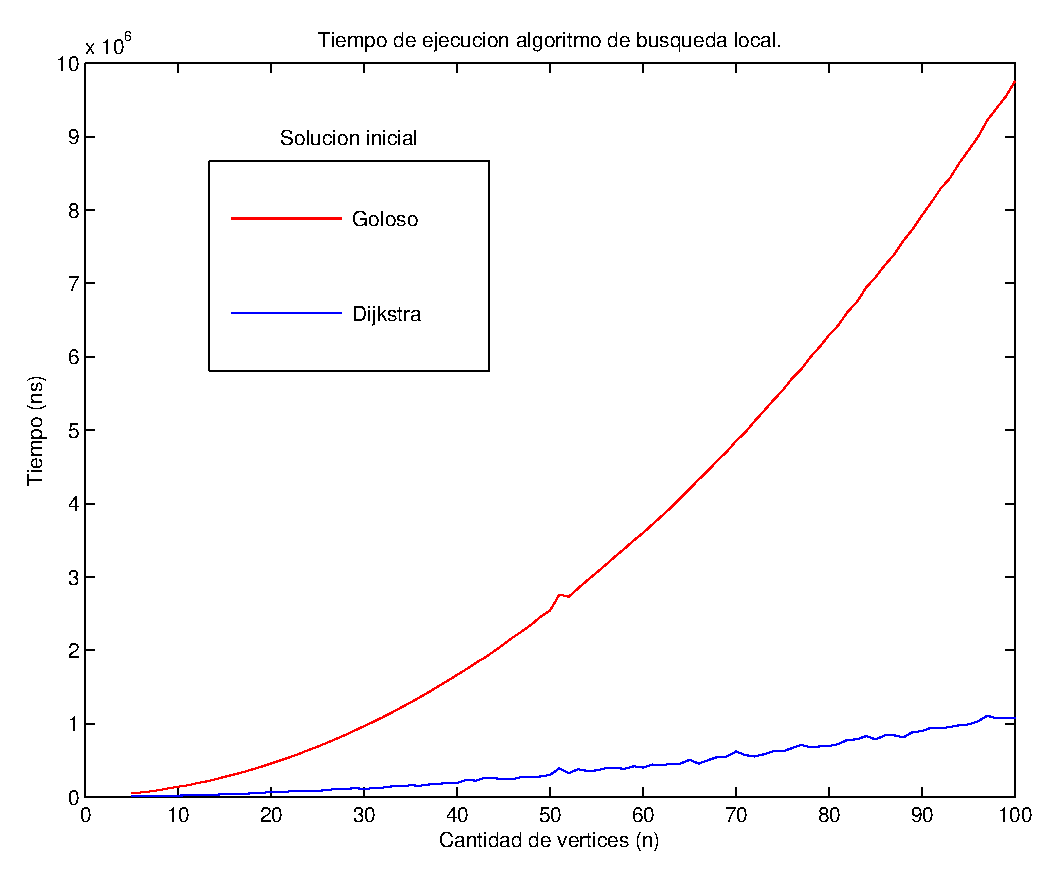
\includegraphics[width=\linewidth]{graficos/busq_local_tiempo.eps}
    \caption{Tiempo ejecución búsqueda local}\label{fig:busq-local-tiempo}
  \end{minipage}
  \hfill
  \begin{minipage}{0.5\linewidth}
    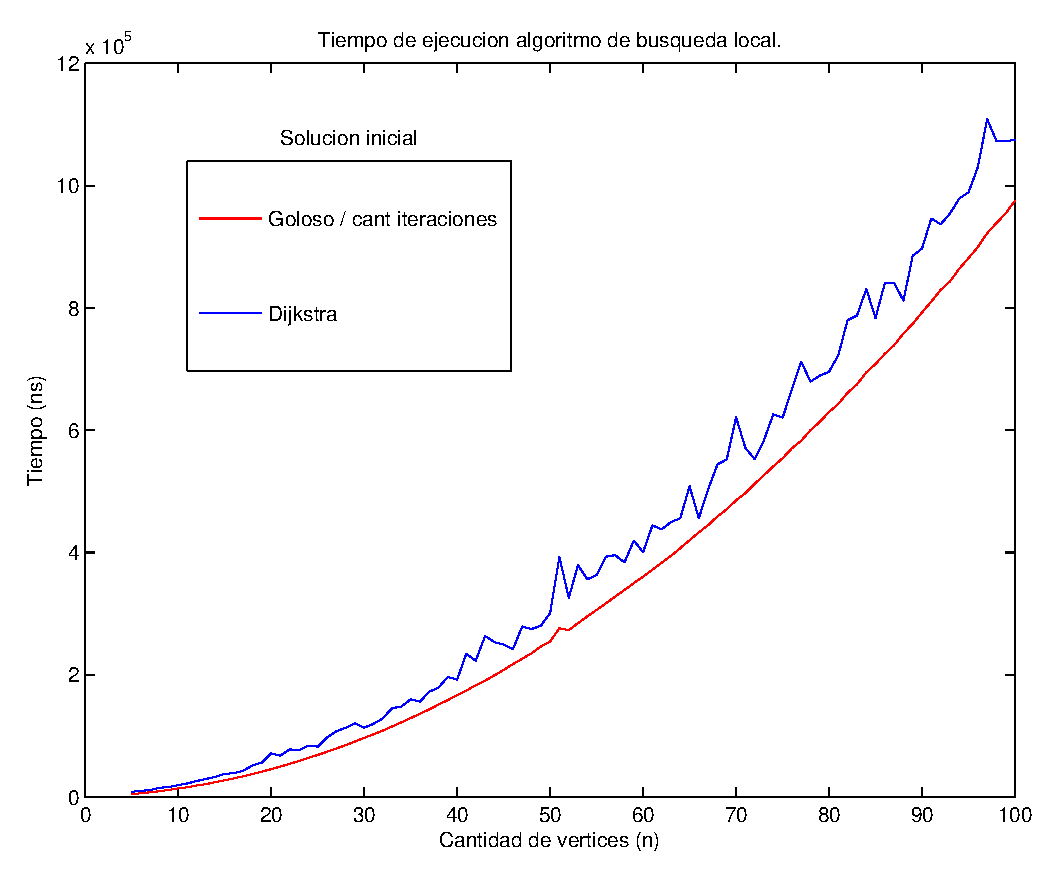
\includegraphics[width=\linewidth]{graficos/busq_local_tiempo_divido10.eps}
    \caption{Idem divido 10}\label{fig:busq-local-tiempo-div10}
  \end{minipage}
\end{figure}

Como podemos observar en el gráfico de la Figura \ref{fig:busq-local-tiempo} el algoritmo de búsqueda local utilizando nuestro algoritmo goloso tiene un tiempo de ejecución mayor al que utiliza el algoritmo de Dijkstra. Esto se debe a que lo que medimos es el tiempo en correr primero los algoritmos que generan las soluciones iniciales y luego correr el algoritmo de búsqueda local. Como ya sabemos nuestro algoritmo goloso corre el algoritmo de Dijkstra una cantidad de iteraciones prefijada. Resulta lógico pensar que un algoritmo que corre el algoritmo de Dijkstra muchas veces tendrá un tiempo de ejecución mayor al de un algoritmo que lo corre sólo una.

Por esto en el gráfico de a Figura \ref{fig:busq-local-tiempo-div10} mostramos los mismos tiempos que en el otro gráfico pero dividimos el tiempo que tarda el algoritmo de búsqueda local que usa nuestro algoritmo goloso por \emph{cant iteraciones}. Con este gráfico, logramos ver que el tiempo de ejecución de ambos algoritmos de búsqueda es parecido cuando reducimos el factor de tiempo de ejecución del algoritmo nos da la solución inicial.

A continuación incluimos unos gráficos que comparan la calidad de las soluciones del algoritmo de búsqueda local.

\begin{figure}[H]
  \begin{minipage}{0.5\linewidth}
    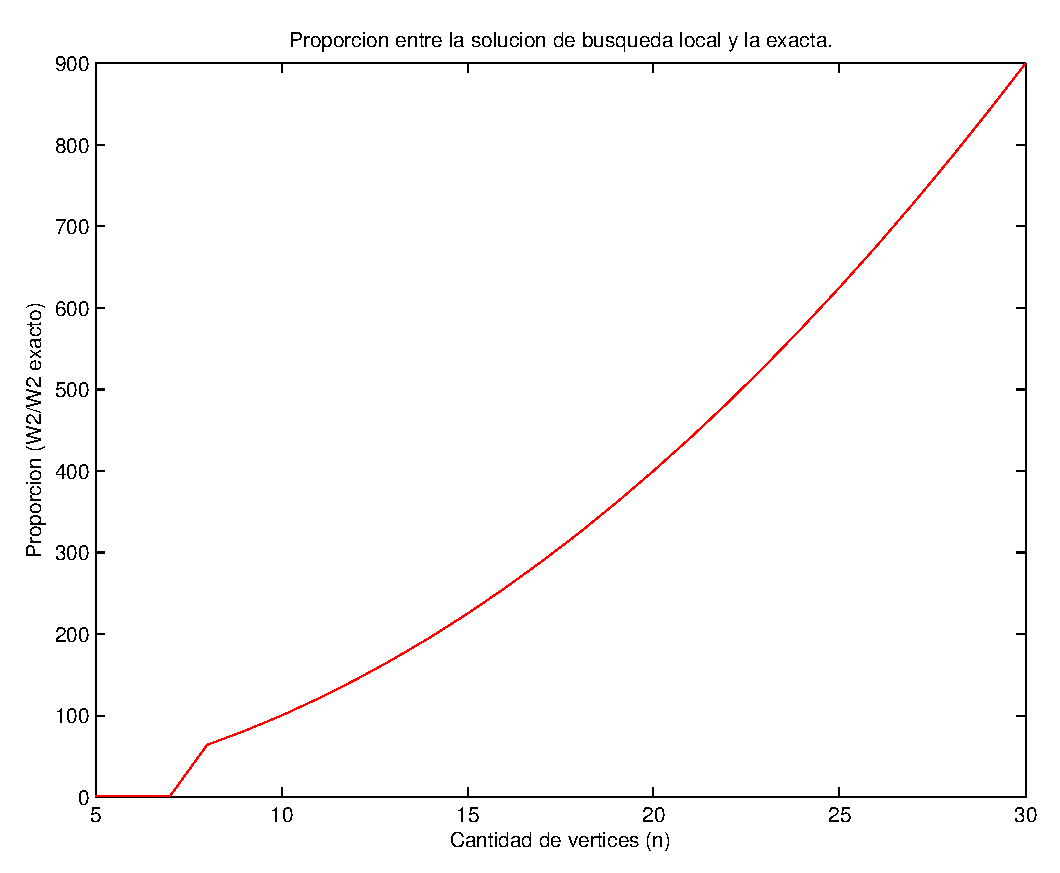
\includegraphics[width=\linewidth]{graficos/busq_local_proporcion.eps}
    \caption{Diferencia proporcional busqueda/exacto}\label{fig:busq-local-proporcion}
  \end{minipage}
  \hfill
  \begin{minipage}{0.5\linewidth}
    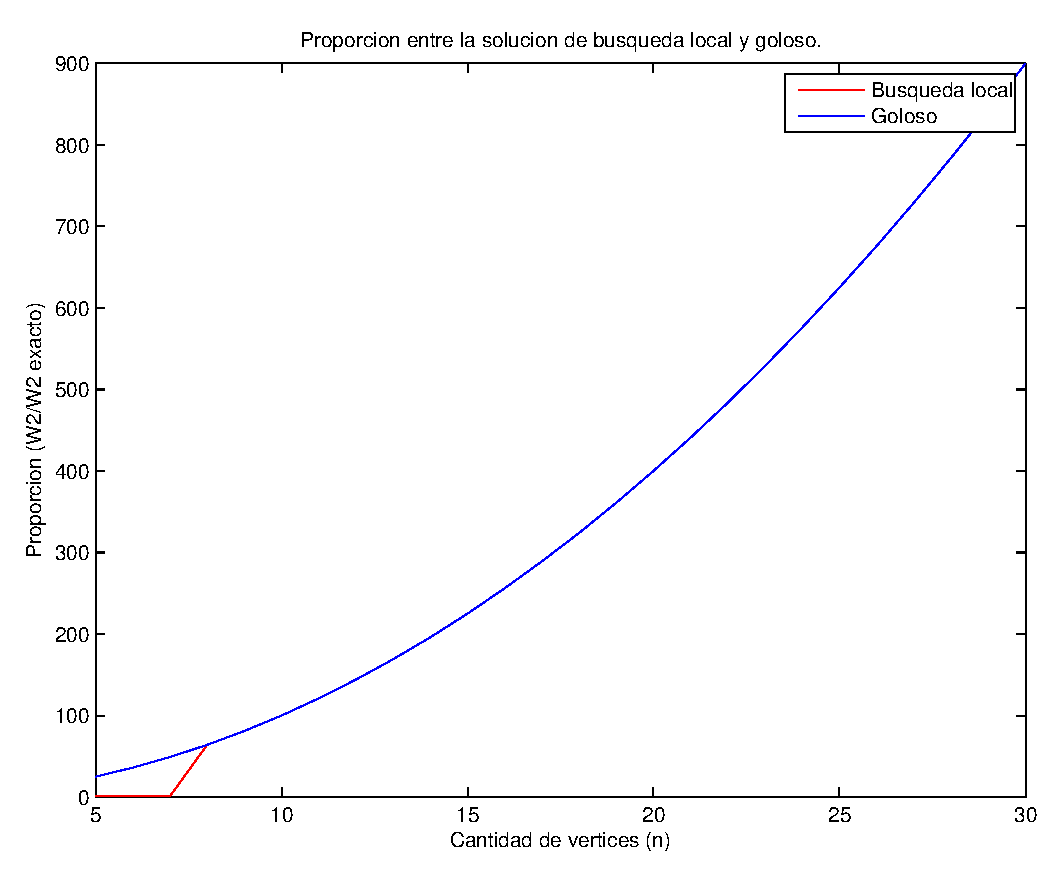
\includegraphics[width=\linewidth]{graficos/busq_local_proporcion_comparacion.eps}
    \caption{Calidad Soluciones Goloso/Dijkstra en familia \emph{3-caminos}}\label{fig:busq-local-proporcion-comparacion}
  \end{minipage}
\end{figure}

El gráfico de la Figura \ref{fig:busq-local-proporcion} muestra la diferencia proporcional entre las soluciones que nos da el algoritmo de búsqueda local con una solución inicial dada por nuestro algoritmo goloso y el algoritmo exacto para la familia de grafos que rompe nuestro algoritmo goloso \emph{3-caminos}. El gráfico de la Figura \ref{fig:busq-local-proporcion-comparacion} compara la proporción con respecto al algoritmo exacto de las soluciones dadas por el algoritmo goloso y las soluciones resultantes de aplicar búsqueda local tomando como soluciones iniciales a las soluciones dadas por el algoritmo goloso para la misma familia de grafos del gráfico de la Figura \ref{fig:busq-local-proporcion}. Mostramos esto en dos gráficos distintos para que se logre apreciar que para la mayoría de los casos, el algoritmo de búsqueda local no logra mejorar las soluciones del nuestro algoritmo goloso para esta familia.

Vale aclarar que en este experimento pudimos correr el algoritmo exacto para grafos con una cantidad de nodos un poco mayor que en las anteriores mediciones. Esto se debe a que para esta familia de grafos el algoritmo exacto tarda menos tiempo en correr ya que hay menos caminos que revisar (recordemos que los grafos de nuestra familia se componen de tres caminos disjuntos en aristas).

Como podemos observar para $n \leq 7$ el algoritmo de búsqueda local logra mejorar la calidad de la solución dada por el nuestro algoritmo goloso. Sin embargo, cuando $n > 7$ no logra mejorarla. Esto verifica lo que dijimos en la sección \ref{subsub:algoritmos-heuristicos-busqueda-calidad.tex}.

Para continuar experimentando, incluimos un gráfico que muestre como se comporta nuestro algoritmo de búsqueda local ante grafos que sean de la familia \emph{3-caminos con puentes} definida en la sección \ref{subsub:algoritmos-heuristicos-busqueda-calidad.tex}. 

\begin{figure}[H]
  \begin{center}
    \begin{minipage}{0.5\linewidth}
      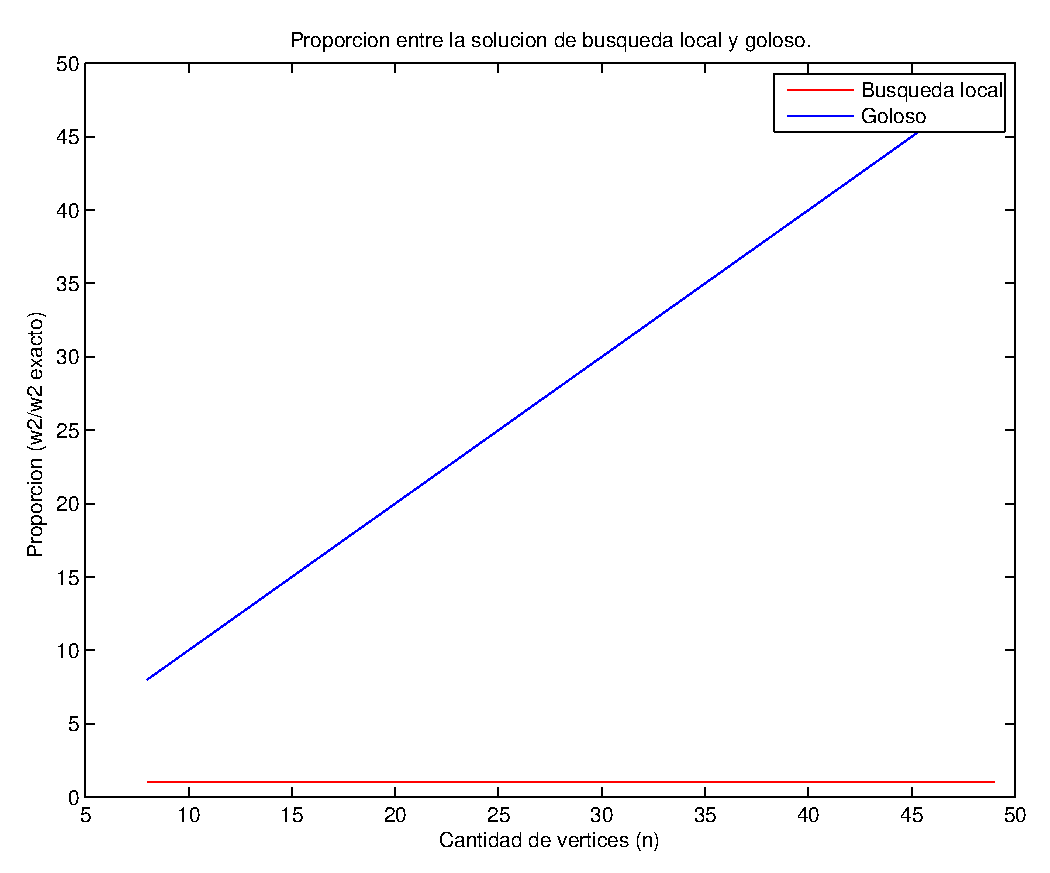
\includegraphics[width=\linewidth]{graficos/busq_local_proporcion2.eps}
      \caption{Calidad Soluciones Goloso/Dijkstra en familia \emph{3-caminos con puentes}}\label{fig:busq-local-proporcion-2}
    \end{minipage}
  \end{center}
\end{figure}

En el gráfico podemos observar el comportamiento del algoritmo de búsqueda local en proporción al algoritmo exacto comparado al comportamiento del algoritmo goloso, también en proporción. Como podemos observar en esta familia el algoritmo de búsqueda local sí puede mejorar la solución que el algoritmo goloso le da como inicial. Más aún, el grafico nos permite observar que no sólo las mejora, sino que logra encontrar la solución óptima, ya que como vemos el peso $W2$ de la solución dada por dicho algoritmo es igual al del de la solución del algoritmo exacto. Esto verifica lo que dijimos en la sección \ref{subsub:algoritmos-heuristicos-busqueda-calidad.tex}.

A continuación incluiremos un gráfico que compara la calidad de las soluciones del algoritmo de busqueda local cuando éste toma como solución inicial la dada por el algoritmo de Dijkstra tomando como función de peso el para las aristas la función $\omega_1$

\begin{figure}[H]
  \begin{center}
    \begin{minipage}{0.5\linewidth}
      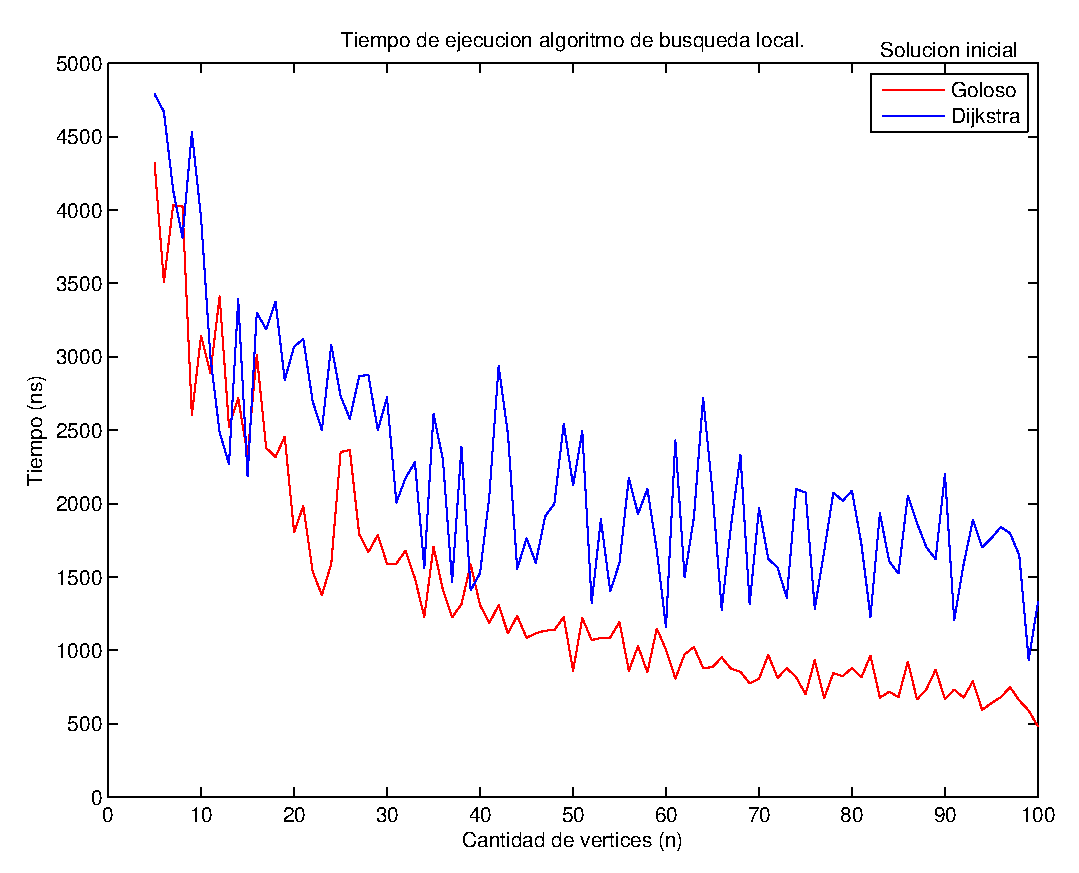
\includegraphics[width=\linewidth]{graficos/busq_local_calidad.eps}
      \caption{Comparacion Soluciones iniciales}\label{fig:busq-local-calidad}
    \end{minipage}
  \end{center}
\end{figure}
  
Como podemos observar en la Figura \ref{fig:busq-local-calidad}, para los grafos con los que hicimos las mediciones, el algoritmo que toma como solución inicial la dada por nuestro algoritmo goloso en general es mejor que la dada por el algoritmo de Dijkstra.

%TODO decir porque es mejor con el goloso
Creemos que esto es así porque, como ya vimos en la sección \ref{subsub:algoritmos-heuristicos-goloso-experimentacion.tex} las soluciones dadas por nuestro algoritmo goloso son mejores que las dadas por el algoritmo de Dijkstra. Una vez que nuestro algoritmo de búsqueda local toma estas soluciones iniciales mejora ambas. Sin embargo, no la logra mejorar lo suficiente las soluciones dadas por el algoritmo de Dijkstra como para que dichas soluciones superen a las dadas por nuestro algoritmo goloso, una vez que son mejoradas por búsqueda local.

Debido a los resultados obtenidos anteriormente, llegamos a la conclusión de que, en general, resulta mejor utilizar nuestro algoritmo goloso para generar las soluciones iniciales que utilizar el algoritmo de Dijkstra tomando $\omega_1$ como función de peso. Por lo tanto, a partir de ahora utilizaremos únicamente nuestro algoritmo goloso para generar las soluciones iniciales para luego aplicarles busqueda local.

\newpage


%%%%%%%%%%%%%%%%%%%%%%%%%%%%%%%%%%%%%%%%%%%%%%%%%%%%%%%%%%%%%%%%%%%%%%%%%%%%%%%
%% Algoritmos heurísticos                                                    %%
%%%%%%%%%%%%%%%%%%%%%%%%%%%%%%%%%%%%%%%%%%%%%%%%%%%%%%%%%%%%%%%%%%%%%%%%%%%%%%%

\section{Algoritmos heurísticos}
\label{sec:algoritmos-heuristicos}

  \subsection{Heuristica constructiva golosa}
  \label{sub:algoritmos-heuristicos-goloso}
      \subsubsection{Desarrollo del algoritmo}
      \label{subsub:algoritmos-heuristicos-goloso-desarrollo.tex}
      En esta sección describiremos detalladamente el diseño de nuestro algoritmo de búsqueda local. 

\subsubsection{Vecindad}

La escencia de este algoritmo se encuentra principalmente en la vecindad que elegimos para las posibles soluciones, a continuación la detallaremos.

Supongamos que tenemos un camino $C$ = ($c_0$, $c_1$, ..., $c_k$) de $k+1$ nodos que es una solución factible del problema de CACM par un grafo $G$ = ($V$,$E$). Los vecinos de la solución $C$ son caminos que también sean soluciones factibles y que surgan de aplicarle una de las siguientes operaciones:

$\bullet$ Quitar Nodo:

Supongamos que existe un $i$ tal que $0 < i < k$ y que ($c_{i+1}$, $c_{i+1}$) $\in$ $E$. Bajo estas condiciones podemos afirmar que existe un camino en $G$ llamado $C'$ tal que $C'$ = ($c_0$, ..., $c_{i-1}$, $c_{i+1}$, ..., $c_k$). Esto significa que dado $C$ podemos eliminar el nodo $c_i$ del camino y unir $c_{i-1}$ y $c_{i+1}$ ya que estos son adyacentes entre sí, obteniendo un camino $C'$ de $k$ nodos.

$\bullet$ Agregar Nodo:

La operación agregar nodo es la operación inversa a la operación Quitar Nodo descripta anteriormente. Supongamos que existe un $i$ tal que $0 \leq i < k$ y existe un nodo $w \in V$ tal que ($c_i$,$w$) $\in E$ y ($w$, $c_{i+1}$) $\in E$. En este caso podemos afirmar que podemos construir un camino $C'$ = ($c_0$, ..., $c_{i}$,$w$,$c_{i+1}$) de $k+2$ nodos.

Vale aclarar que para realizar esta operación, el nodo $w$ no debe pertenecer a $C$, ya que queremos que el camino sea simple.

$\bullet$ Cambiar Nodo:

Esta operación es una mezcla de las dos operaciones anteriores. Supongamos que existe un $i$ tal que $0 \leq i < k-1$ y que existe un nodo $w \in V$ (nuevamente, $w$ no debe estar en el camino $C$) tal que ($c_i$,$w$) $\in E$ y ($w$, $c_{i+2}$) $\in E$. En este caso podemos cambiar el nodo $c_{i+1}$ del camino $C$ por el nodo $w$ obteniendo un nuevo camino $C'$ de la misma cantidad de nodos.

Uno podría creer que la operación Cambiar Nodo es una combinación de las dos operaciones descriptas anteriormente Agregar Nodo y Quitar Nodo, ya que se podría quitar primero el nodo $c_{i+1}$ y luego agregar el nodo $w$. Sin embargo, esto no es así ya que podría pasar que el eje ($c_i$,$c_{i+2}$) $\notin E$ y, si esto ocurre no nos sería posible quitar el nodo $c_{i+1}$ para luego agregar el nodo $w$.

Dadas estas tres operaciones, un vecino de una solución factible $C$ es un camino que se pueda construir aplicándole a $C$ una de estas tres operaciones. Nótese que si existiese un $C'$ que se pudiera construir a partir de aplicarle a $C$ más de una operación, $C'$ no sería vecino de $C$. Tomamos esta decisión debido a que pensamos que si consideráramos vecino a un camino que se pudiera construir a partir de aplicarle numerosas operaciones a $C$ se estaría perdiendo, por así decirlo, la localidad de la búsqueda y estaríamos incurriendo en una búsqueda más global. Es importante recalcar que sólo tomamos como un vecino de $C$ un camino $C'$ factible.

Algo que pensamos mientras elegíamos nuestra vecindad es que una buena propiedad que ésta pudiese cumplir sería que, dada una solución factible $C$, aplicándole una cantidad de operaciones, pudiésemos llegar a cualquier otra solución factible.

Para explicar esto pensemos en los números reales. Supongamos tenemos una función $F: \mathbb{R} \Rightarrow \mathbb{R}$ y queremos hallar su máximo mediante una búsqueda local. Para esto podemos elegir, dado un $c \in \mathbb{R}$, una función de vecindad que devuelva por ejemplo el conjunto $[c-\varepsilon, c+\varepsilon]$  para algún $\varepsilon$. Dada esta función de vecindad podemos observar que aplicándola muchas veces nos podemos mover a lo largo de todo el dominio de la función $F$.

Que una función de vecindad cumpla con esta propiedad nos parece bueno porque al poder moverse de cualquier solución factible a cualquier otra, nos garantizamos de que no habrá soluciones factibles buenas que nos estemos perdiendo. Más aún, si esta propiedad vale podemos afirmar que si aplicamos muchas veces la función de vecindad (empezando de una solución $C$ luego en un vecino de $C$ y así) eventualmente podemos llegar a la solución óptima del problema (aunque probablemente sea necesario aplicar esta función un número inmenso de veces para llegar y no se estaría haciendo búsqueda local).

Luego de pensarlo llegamos a la conclusión de que nuestra vecindad no cumple con esa propiedad, ya que existen casos en los que a partir de una solución nos es imposible llegar a otra.

Supongamos que nuestro grafo es $C_n$ y que nuestro nodo inicial es $c_1$ y nuestro nodo destino es $c_n$. Supongamos además que tenemos una solución que es $S$ = ($c_1$, $c_2$, ... , $c_n$). Podemos observar que hay otra posible solución, que es $S'$ = ($c_1$,$c_n$) ya que como nuestro grafo es $C_n$ entonces $c_1$ y $c_n$ están unidos. Sin embargo, con nuestra función de vecindad nos es imposible llegar de la solución $S$ a la solución $S'$. ya que no hay ninguna operación que se pueda realizar a $S$. 

Supongamos ahora que tenemos como solución inicial $S'$. En este caso tampoco podemos aplicar ninguna operación a $S'$ y no podremos llegar a la otra solución. Podemos decir que en este caso, en nuestra vecindad tanto $S$ como $S'$ son soluciones sin vecinos.

Luego de pensar como solucionar este problema, llegamos a la conclusión de que para resolverlo deberíamos tener una vecindad muy grande y perderíamos la localidad de la búsqueda. Por ejemplo, en el caso anterior, para llegar de la solución $S'$ a la solución $S$ una operación debería ser agregar a $S'$ un camino de $n$ nodos, lo cual es fácil para el grafo $C_n$ pero muy complejo para otros grafos.

\subsubsection{Algoritmo}

Habiendo explicado las características de nuestra vecindad, a continuación describiremos el algoritmo de busqueda local.

Nuestro algoritmo recibe como entrada el grafo $G$ y una solución inicial $C$. Luego de esto el algoritmo entra en un ciclo en el que se buscan los vecinos de la mejor solución $S$ que se tenga. Si existe un vecino $S'$ mejor que $S$, entonces la mejor solución pasa a ser $S'$ y pasamos a la siguiente iteración. En la iteración en la que no exista un vecino mejor que $S$ entonces se termina la búsqueda.
%TODO: En realidad búsqueda local siempre es así, deberíamos sacar este párrafo?

A continuación incluiremos un pseudocódigo del algoritmo.
\begin{center}
 \begin{figure}[H]
  \begin{pseudo}
   \Procedure{busqueda local}{grafo G, camino sol}
   \State $mejorSol \leftarrow sol$
   \While{$seguirBuscando$}
      \State $buscarVecinoQuitar(mejorSol, mejorVecino, G)$
      \State $buscarVecinoAgregar(mejorSol, mejorVecino, G)$
      \State $buscarVecinoCambiar(mejorSol, mejorVecino, G)$
      \If{$mejorVecino.W_1 > k \vee mejorVecino.W_1 \geq mejorSol.W_1$}
	\State $seguirBuscando \leftarrow false$
      \Else
	\State $actualizar(mejorSol, mejorVecino)$
      \EndIf
      \State Devolver $mejorSol$
   \EndWhile
   \EndProcedure
  \end{pseudo}
 \end{figure}
\end{center}

En este algoritmo usamos la estructura Camino, que es una lista de ejes y además tiene el peso total $W_1$ y $W_2$. Y además usamos la estructura vecino, que tiene tres tipos: $TIPO1$ significa que es un vecino que surge de eliminar un nodo de la solución actual, $TIPO2$ que surge de agregar un nodo, o $TIPO3$, que surge de cambiar un nodo por otro. Además la estructura tiene una posición donde hay que hacer los cambios para pasar del camino actual al vecino (estos cambios se deducen según el tipo del vecino que sea). Por último la estructura cuenta con una lista de nodos a agregar al camino actual, si se cambia o agrega un nodo la lista tendrá un elemento y si se elimina un nodo la lista será vacía.

Utilizamos esta estructura para poder pasar de un camino a su vecino en una complejidad constante ya que ésta cuenta con la información necesaria para saber cuáles son los cambios a realizar y dónde hay que realizarlos. Si no contáramos con esta estructura y tuviésemos simplemente otro camino deberíamos copiar el camino para actualizar la solución, lo que tendría una complejidad temporal lineal.

      \subsubsection{Complejidad temporal de peor caso}
      \label{subsub:algoritmos-heuristicos-goloso-complejidad.tex}
      \begin{center}
 \begin{figure}[H]
  \begin{pseudo}
   \Procedure{cacm\_goloso}{grafo $G$, nodo $u$, nodo $v$}
    \State $pInicial \leftarrow 0$, $pFinal \leftarrow 1$, $pMedio$ \Ode{1}
    \For{$i < Cant\_Iteraciones$}
      \State $pMedio \leftarrow (pInicial + pFinal)/2$ \Ode{1}
      \State $solucion$ $\leftarrow$ $Dijkstra(G$, $pMedio$, $u$, $v)$ \Ode{n^2}
      \If{$W_1(solucion) \leq k$} \Ode{1}
	 \State $pInicial \leftarrow pMedio$ \Ode{1}
      \Else
	 \State $pFinal \leftarrow pMedio$ \Ode{1}
      \EndIf
    \EndFor
    \If{$W_1(solucion) \leq k$} \Ode{1}
      \State $solucion \leftarrow Dijkstra(G, 1)$ \Ode{n^2}
    \EndIf
    \State Devolver solución \Ode{1}
   \EndProcedure
  \end{pseudo}
 \end{figure}
\end{center}

 Como podemos ver el algoritmo esta compuesto por una instrucción $O(1)$ luego un for,y por ultimo 2 $O(1)$ y una vez Dijkstra, que como sabemos tiene complejidad $O(n^2)$. El for itera $Cant\_Iteraciones$ instrucciones $4*O(1) + O(n^2)$. Como $Cant\_Iteraciones$ es un numero acotado, la complejidad del for es $O(n^2)$. Por álgebra de ordenes $O(1)+O(n^2)+2*O(1)+O(n^2)=O(n^2)$.  

      \subsubsection{Análisis de la calidad de las soluciones}
      \label{subsub:algoritmos-heuristicos-goloso-calidad.tex}
      Para probar que nuestro algoritmo no siempre da la solucion optima, vamos a presentar una familia que no solo nuestro algoritmo no encuentra la cota, sino tambien demostramos que no es \emph{k-acotado}, para ningun $k$ finito.

%TODO crear y agregar figura q represente la familia

$G_n$ esta compuesto por n nodos que se dividen en tres camino simples entre los nodos $1$ y $n$. A estos caminos los llamaremos $a$, $b$ y $c$ repectivamente. Los nodos se dividiran indiferentemente entre estos 3 caminos, pero cumpliendo que el costo total de cada camino sera:

$\bullet$ $W_1(a) = k+1$, $W_2(a)=1$

$\bullet$ $W_1(b) = k$, $W_2(b)=Q$

$\bullet$ $W_1(c) = 1$, $W_2(c)=i*Q$

Con $k$ la cota sobre $W_1$, $i$ sera la proporcion entre el resultado de nuestro algoritmo y el optimo y $Q$ sera seleccionado para cumplir la condicion anterior.

La idea de esta familia es que $a$ sea un camino donde se supera la cota por muy poco, pero tenga un $W_2$ muy bajo, $b$ sea el camino optimo y su valor de $W_1$ sea exactamente $k$ y $c$ sea el camino que encuentra nuestro algoritmo, que tiene un $W_1$ muy bajo pero $W_2 = i * W_2(b)$.

Esto va a suceder ya que no va a existir ningun $p$ para el cual el camino $b$ sea mejor que los otros dos al mismo tiempo. Para $p$ muy chiquitos $b$ sera mejor que $a$ y para $p$ muy grandes sera mejor que $c$. Claramente si se cumple lo anterior no abra ningun $p$ que sea mejor que ambas.

\textbf{Demostracion:}

Primero veamos como tiene que ser $p$ para que $b$ sea menor que $a$.

Sea $p$ tal que 

$(1-p)*W_1(b)+p*W_2(b) < (1-p)*W_1(a)+p*W_2(a)$

$(1-p)*k+p*Q < (1-p)*(k+1)+p$

$k-p*k+p*Q < k-p*k-p+1+p$

$p*Q < 1$

$p < \frac{1}{Q}$ Para que $b$ sea mejor que $a$

Ahora veamos como tiene que ser $p$ para que $b$ sea menor que $c$.

Sea $p$ tal que 

$(1-p)*W_1(b)+p*W_2(b) < (1-p)*W_1(c)+p*W_2(c)$

$(1-p)*k+p*Q < (1-p)+p*i*Q$

$k-p*k+p*Q < 1-p+p*i*Q$

$k-1 < -p+p*i*Q+p*k-p*Q$

$k-1 < p*(-1+i*Q+k-Q)$

$\frac{k-1}{-1+i*Q+k-Q} < p$ Tomando $k,i > 1$, ya que $k > 1$ y $Q*i > Q \rightarrow i*Q-Q+k-1 > 0$ por $Q > 0$

Para que $b$ sea mejor que $a$ y $c$ se deberia cumplir:

$\frac{k-1}{-1+i*Q+k-Q} < p < \frac{1}{Q}$

Para forzar que esto no ocurra buscamos $k$ y $Q$ tal que:

$\frac{k-1}{i*Q-Q+k-1} > \frac{1}{Q}$

$k-1 > \frac{i*Q-Q+k-1}{Q}$ ya que $i*Q-Q+k-1 > 0$ como vimos en el punto anterior

$k-1 > \frac{k-1}{Q}+i-1$

$(k-1) \frac{Q-1}{Q} > i-1$

Tomando $Q=3$ y $k=2*i-1$

$(2*i-2) \frac{2}{3} > i-1$

$(i-1) \frac{4}{3} > i-1$

$(i-1) \frac{1}{3} > 0$

$i-1 > 0$

$i > 1$ Como ya habiamos dicho antes.


O sea la familia para un $n$ y un $i$ dado estaria conformada por:

$k = 2*i-1$

$\bullet$ $W_1(a) = 2*i$, $W_2(a)=1$

$\bullet$ $W_1(b) = 2*i-1$, $W_2(b)=3$

$\bullet$ $W_1(c) = 1$, $W_2(c)=i*3$

Veamos que para cualquier $i$, la proporcion entre el camino encontrado en la golosa y el exacto es $i$:

Como demostramos previamente nuestro algoritmo va a encontrar el camino $c$ que tiene $W_2=i*3$, y el camino oprtimo es el $b$, con $W_2=3$. Por los que claramente la propocion es $i$, $\frac{3i}{3}=i$.

Para armar un grafo de esta familia hay diversas formas.Siempre se fijan 2 nodos como el inicial y el final. Los demas nodos se distribuyen entre tres caminos disjuntos en nodos, de forma arbitraria. Particularmente nuestra implementación distribuimos equitativamente los nodos entre los 3 caminos. (Los nodos sobrantes , $(n-2) mod 3$, los dejamos como nodos aislados por un tema de facilidad).

Luego queda asignar los pesos a las aristas, hay que distribuir el peso de cada camino entre las aristas del mismo. Otra vez esto puede hacerse arbitrariamente, y en nuestro caso buscamos una distribución uniforme.
En el caso de pesos reales, se divide el peso total del camino por la cantidad de aristas y se asigna ese peso a cada arista.
En el caso de pesos enteros esto no se puede realizar porque no podemos asegurar que sea dividible. Para asegurarnos multiplicamos los pesos de los 3 caminos por la cantidad de aristas de un camino (las 3 tienen la misma cantidad) para asegurarnos que sea dibidible. Esto no afecta nada del analisis anteror ya que al multiplicar a todos los caminos por un mismo número no afecta ni la elección del algoritmo ni la proporción.

Cabe aclarar que esta familia se puede extender agregando cualquier cantidad de nodos y aristas arbitrarias, siempre y cuando el camino $b$ siga siendo el único óptimo. En esta extención el goloso nunca encontrará el óptimo ya que al agregar otras opciones no afecta que no exista ningun $p$ para el cual el camino $b$ (óptimo) sea mejor que todos los demas, ya que no puede ser mejor que $a$ y $c$ al mismo tiempo. Pero al extender la familia lo que si se pierde es el analisis de	qué tan mala puede ser la solución.  

      \subsubsection{Experimentación}
      \label{subsub:algoritmos-heuristicos-goloso-experimentacion.tex}
      En esta sección, realizaremos diversos experimentos para verificar tanto el tiempo de ejecución como la calidad de las soluciones de nuestro algoritmo de búsqueda local.

Como dijimos anteriormente, el algoritmo de búsqueda local toma una solución inicial. Nosotros tomamos como un parámetro del algoritmo la solución inicial que éste recibe.

En los gráficos que presentamos a continuación, mostramos el tiempo de ejecución de correr búsqueda local con dos algoritmos que nos dan soluciones iniciales. Un algoritmo es el algoritmo goloso que detallamos en la sección \ref{subsub:algoritmos-heuristicos-goloso-desarrollo.tex}, y el otro es el algoritmo de Dijkstra tomando como pesos de las aristas la función $\omega_1$.

\begin{figure}[H]
  \begin{minipage}{0.5\linewidth}
    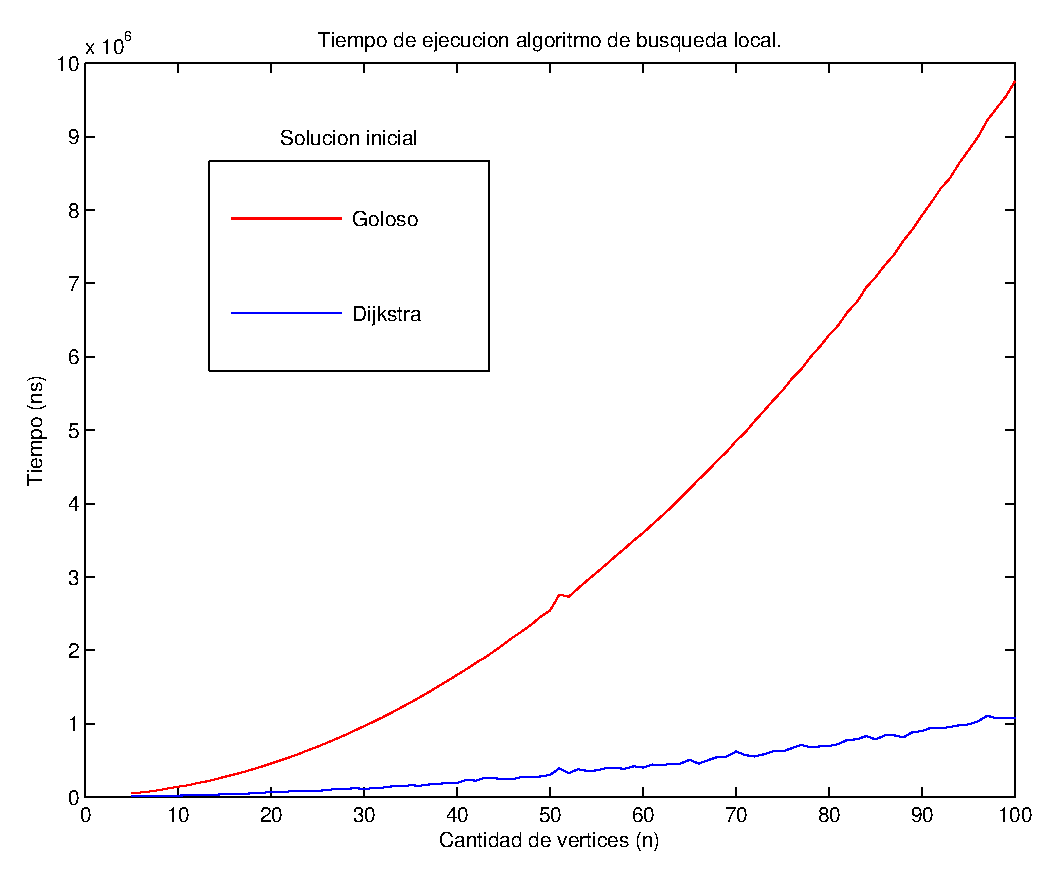
\includegraphics[width=\linewidth]{graficos/busq_local_tiempo.eps}
    \caption{Tiempo ejecución búsqueda local}\label{fig:busq-local-tiempo}
  \end{minipage}
  \hfill
  \begin{minipage}{0.5\linewidth}
    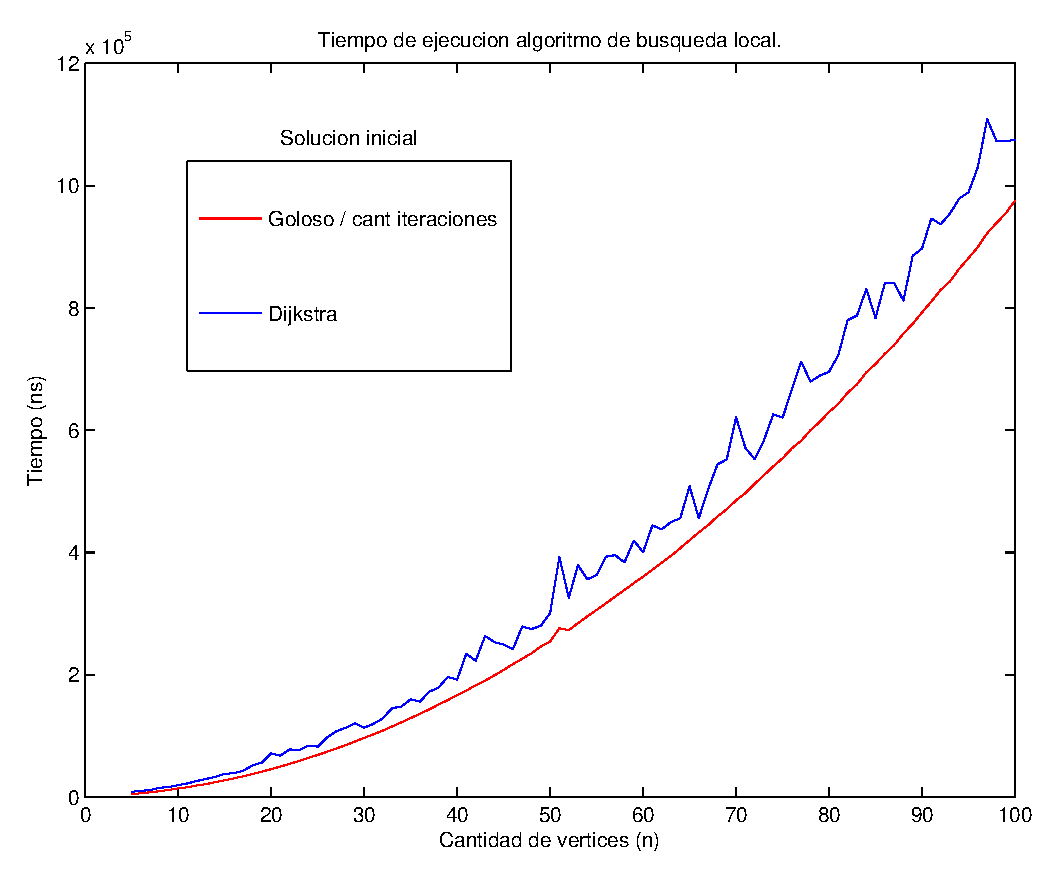
\includegraphics[width=\linewidth]{graficos/busq_local_tiempo_divido10.eps}
    \caption{Idem divido 10}\label{fig:busq-local-tiempo-div10}
  \end{minipage}
\end{figure}

Como podemos observar en el gráfico de la Figura \ref{fig:busq-local-tiempo} el algoritmo de búsqueda local utilizando nuestro algoritmo goloso tiene un tiempo de ejecución mayor al que utiliza el algoritmo de Dijkstra. Esto se debe a que lo que medimos es el tiempo en correr primero los algoritmos que generan las soluciones iniciales y luego correr el algoritmo de búsqueda local. Como ya sabemos nuestro algoritmo goloso corre el algoritmo de Dijkstra una cantidad de iteraciones prefijada. Resulta lógico pensar que un algoritmo que corre el algoritmo de Dijkstra muchas veces tendrá un tiempo de ejecución mayor al de un algoritmo que lo corre sólo una.

Por esto en el gráfico de a Figura \ref{fig:busq-local-tiempo-div10} mostramos los mismos tiempos que en el otro gráfico pero dividimos el tiempo que tarda el algoritmo de búsqueda local que usa nuestro algoritmo goloso por \emph{cant iteraciones}. Con este gráfico, logramos ver que el tiempo de ejecución de ambos algoritmos de búsqueda es parecido cuando reducimos el factor de tiempo de ejecución del algoritmo nos da la solución inicial.

A continuación incluimos unos gráficos que comparan la calidad de las soluciones del algoritmo de búsqueda local.

\begin{figure}[H]
  \begin{minipage}{0.5\linewidth}
    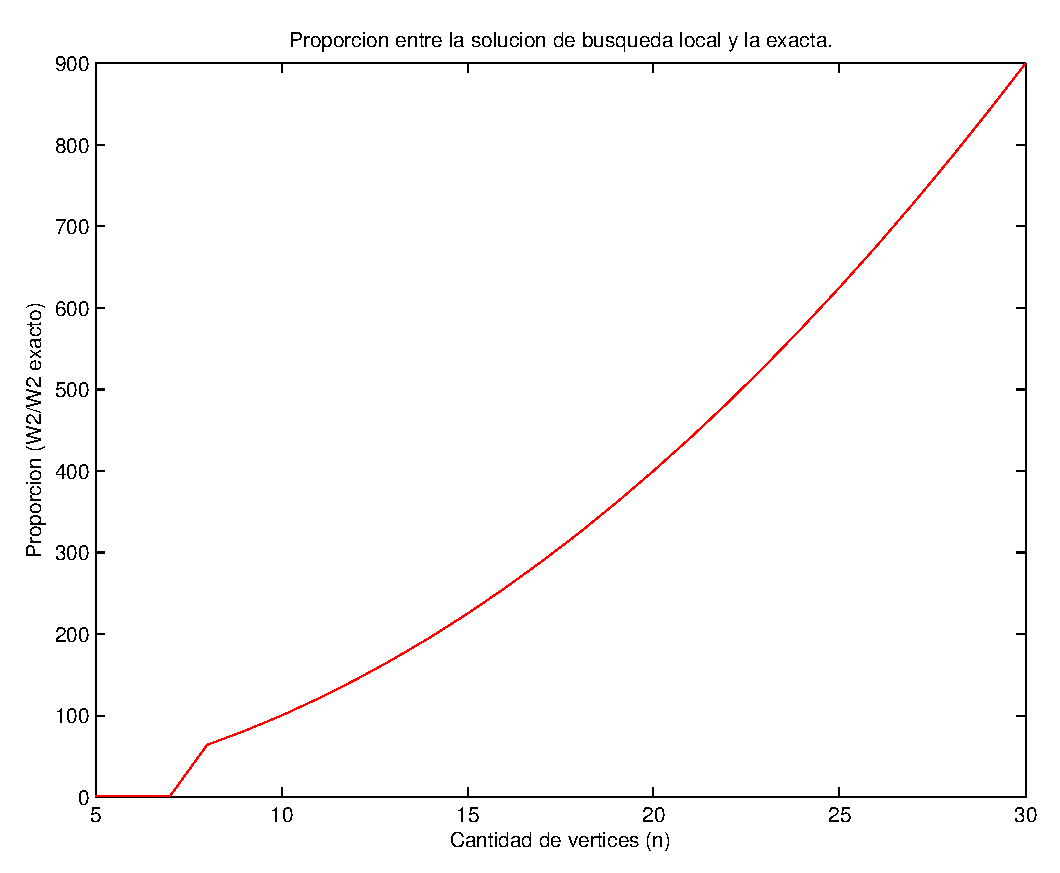
\includegraphics[width=\linewidth]{graficos/busq_local_proporcion.eps}
    \caption{Diferencia proporcional busqueda/exacto}\label{fig:busq-local-proporcion}
  \end{minipage}
  \hfill
  \begin{minipage}{0.5\linewidth}
    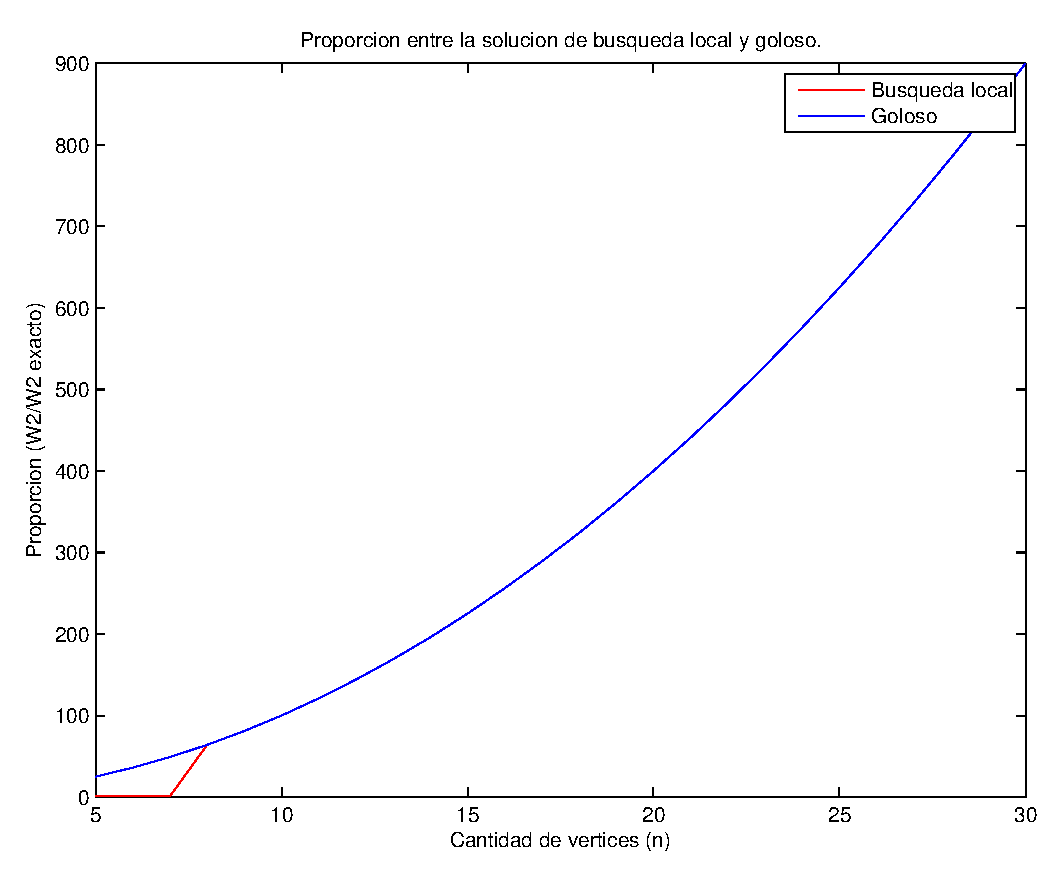
\includegraphics[width=\linewidth]{graficos/busq_local_proporcion_comparacion.eps}
    \caption{Calidad Soluciones Goloso/Dijkstra en familia \emph{3-caminos}}\label{fig:busq-local-proporcion-comparacion}
  \end{minipage}
\end{figure}

El gráfico de la Figura \ref{fig:busq-local-proporcion} muestra la diferencia proporcional entre las soluciones que nos da el algoritmo de búsqueda local con una solución inicial dada por nuestro algoritmo goloso y el algoritmo exacto para la familia de grafos que rompe nuestro algoritmo goloso \emph{3-caminos}. El gráfico de la Figura \ref{fig:busq-local-proporcion-comparacion} compara la proporción con respecto al algoritmo exacto de las soluciones dadas por el algoritmo goloso y las soluciones resultantes de aplicar búsqueda local tomando como soluciones iniciales a las soluciones dadas por el algoritmo goloso para la misma familia de grafos del gráfico de la Figura \ref{fig:busq-local-proporcion}. Mostramos esto en dos gráficos distintos para que se logre apreciar que para la mayoría de los casos, el algoritmo de búsqueda local no logra mejorar las soluciones del nuestro algoritmo goloso para esta familia.

Vale aclarar que en este experimento pudimos correr el algoritmo exacto para grafos con una cantidad de nodos un poco mayor que en las anteriores mediciones. Esto se debe a que para esta familia de grafos el algoritmo exacto tarda menos tiempo en correr ya que hay menos caminos que revisar (recordemos que los grafos de nuestra familia se componen de tres caminos disjuntos en aristas).

Como podemos observar para $n \leq 7$ el algoritmo de búsqueda local logra mejorar la calidad de la solución dada por el nuestro algoritmo goloso. Sin embargo, cuando $n > 7$ no logra mejorarla. Esto verifica lo que dijimos en la sección \ref{subsub:algoritmos-heuristicos-busqueda-calidad.tex}.

Para continuar experimentando, incluimos un gráfico que muestre como se comporta nuestro algoritmo de búsqueda local ante grafos que sean de la familia \emph{3-caminos con puentes} definida en la sección \ref{subsub:algoritmos-heuristicos-busqueda-calidad.tex}. 

\begin{figure}[H]
  \begin{center}
    \begin{minipage}{0.5\linewidth}
      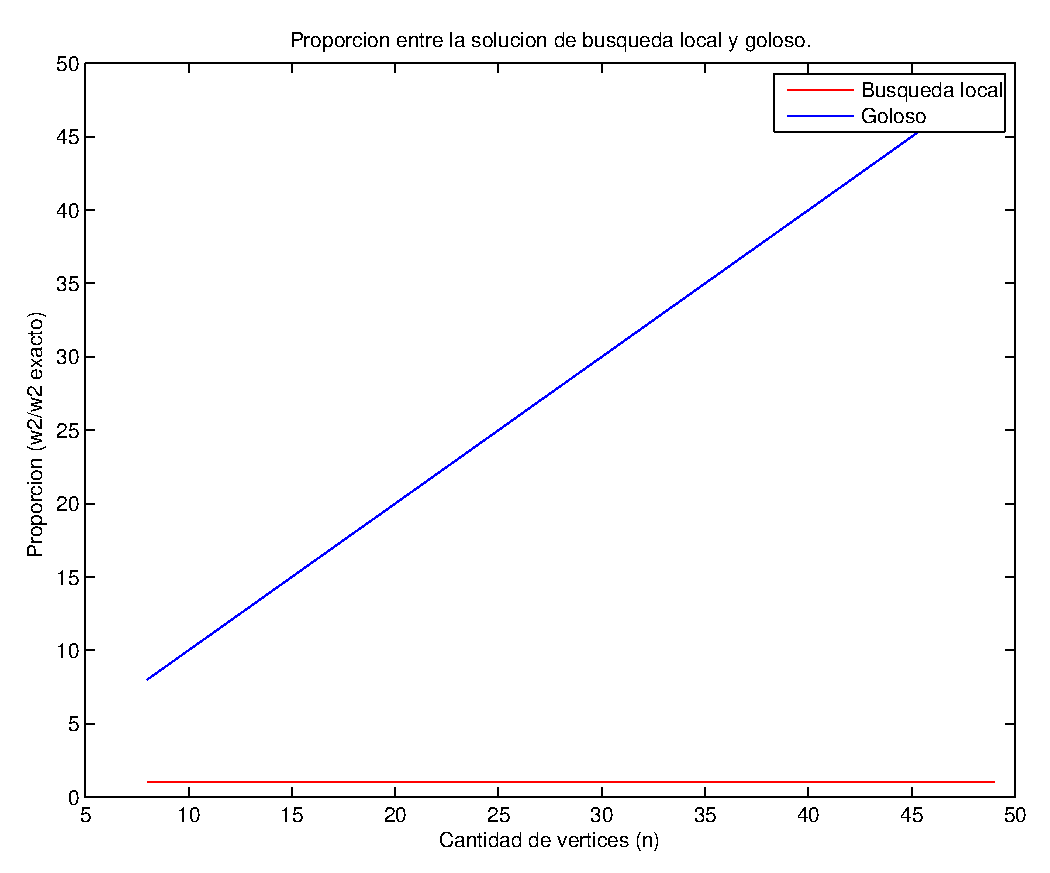
\includegraphics[width=\linewidth]{graficos/busq_local_proporcion2.eps}
      \caption{Calidad Soluciones Goloso/Dijkstra en familia \emph{3-caminos con puentes}}\label{fig:busq-local-proporcion-2}
    \end{minipage}
  \end{center}
\end{figure}

En el gráfico podemos observar el comportamiento del algoritmo de búsqueda local en proporción al algoritmo exacto comparado al comportamiento del algoritmo goloso, también en proporción. Como podemos observar en esta familia el algoritmo de búsqueda local sí puede mejorar la solución que el algoritmo goloso le da como inicial. Más aún, el grafico nos permite observar que no sólo las mejora, sino que logra encontrar la solución óptima, ya que como vemos el peso $W2$ de la solución dada por dicho algoritmo es igual al del de la solución del algoritmo exacto. Esto verifica lo que dijimos en la sección \ref{subsub:algoritmos-heuristicos-busqueda-calidad.tex}.

A continuación incluiremos un gráfico que compara la calidad de las soluciones del algoritmo de busqueda local cuando éste toma como solución inicial la dada por el algoritmo de Dijkstra tomando como función de peso el para las aristas la función $\omega_1$

\begin{figure}[H]
  \begin{center}
    \begin{minipage}{0.5\linewidth}
      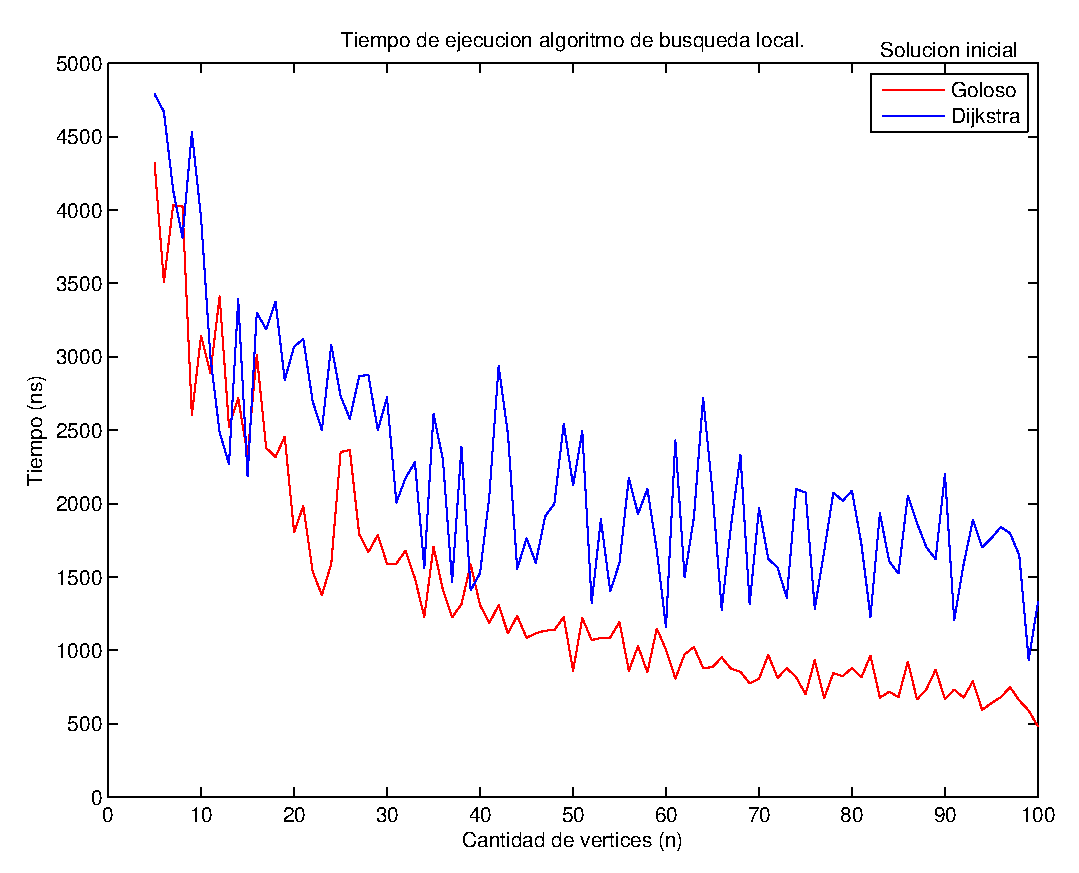
\includegraphics[width=\linewidth]{graficos/busq_local_calidad.eps}
      \caption{Comparacion Soluciones iniciales}\label{fig:busq-local-calidad}
    \end{minipage}
  \end{center}
\end{figure}
  
Como podemos observar en la Figura \ref{fig:busq-local-calidad}, para los grafos con los que hicimos las mediciones, el algoritmo que toma como solución inicial la dada por nuestro algoritmo goloso en general es mejor que la dada por el algoritmo de Dijkstra.

%TODO decir porque es mejor con el goloso
Creemos que esto es así porque, como ya vimos en la sección \ref{subsub:algoritmos-heuristicos-goloso-experimentacion.tex} las soluciones dadas por nuestro algoritmo goloso son mejores que las dadas por el algoritmo de Dijkstra. Una vez que nuestro algoritmo de búsqueda local toma estas soluciones iniciales mejora ambas. Sin embargo, no la logra mejorar lo suficiente las soluciones dadas por el algoritmo de Dijkstra como para que dichas soluciones superen a las dadas por nuestro algoritmo goloso, una vez que son mejoradas por búsqueda local.

Debido a los resultados obtenidos anteriormente, llegamos a la conclusión de que, en general, resulta mejor utilizar nuestro algoritmo goloso para generar las soluciones iniciales que utilizar el algoritmo de Dijkstra tomando $\omega_1$ como función de peso. Por lo tanto, a partir de ahora utilizaremos únicamente nuestro algoritmo goloso para generar las soluciones iniciales para luego aplicarles busqueda local.
  \newpage

  \subsection{Heuristica de busqueda local}
  \label{sub:algoritmos-heuristicos-busqueda}
      
      \label{subsub:algoritmos-heuristicos-busqueda-introduccion_busqueda.tex}
      En esta sección, implementaremos un algoritmo que utilice la técnica de \emph{búsqueda local}. Para hacer este algoritmo definimos un conjunto de soluciones vecindad para cada solución factible del problema. Luego, un algoritmo de búsqueda local toma una solución factible $S$ del problema a resolver como solución inicial y mejora dicha solución recorriendo en forma iterativa los vecinos de $S$ y reemplazándolo cuando encuentra un vecino mejor. El algoritmo realiza este procedimiento hasta encontrar una solución que no tenga ningún vecino que sea mejor, es decir, hasta encontrar un máximo local.

Básicamente, un algoritmo de búsqueda local debería cumplir con el siguiente pseudocódigo, sea $N(S)$ el conjunto de vecinos de la solución $S$ y $f$ la función objetivo que se quiere minimizar:

\begin{center}
 \begin{figure}[H]
  \begin{pseudo}
   \Procedure{busquedaLocal}{}
   \State Sea $S$ una solución inicial
   \While{$(\exists S' \in N(S)) f(S')<f(S)$}
      \State $S \leftarrow S'$
   \EndWhile
   \EndProcedure
  \end{pseudo}
 \end{figure}
\end{center}

            
      \subsubsection{Vecindad}
      \label{subsub:algoritmos-heuristicos-busqueda-desarrollo_vecindad.tex}
      La esencia de este algoritmo se encuentra principalmente en la vecindad que elegimos para las posibles soluciones, la cual detallaremos a continuación.

Supongamos que tenemos un camino $C$ = ($c_0$, $c_1$, ..., $c_k$) de $k+1$ nodos que es una solución factible del problema de CACM par un grafo $G$ = ($V$,$E$). Los vecinos de la solución $C$ son caminos que también sean soluciones factibles y que surjan de aplicarle una de las siguientes operaciones:

\begin{itemize}
 \item Quitar Nodo:

  Supongamos que existe un $i$ tal que $0 < i < k$ y que ($c_{i+1}$, $c_{i+1}$) $\in$ $E$. Bajo estas condiciones podemos afirmar que existe un camino en $G$ llamado $C'$ tal que $C'$ = ($c_0$, ..., $c_{i-1}$, $c_{i+1}$, ..., $c_k$). Esto significa que dado $C$ podemos eliminar el nodo $c_i$ del camino y unir $c_{i-1}$ y $c_{i+1}$ ya que estos son adyacentes entre sí, obteniendo un camino $C'$ de $k$ nodos.
  \item Agregar Nodo:

  La operación agregar nodo es la operación inversa a la operación Quitar Nodo descripta anteriormente. Supongamos que existe un $i$ tal que $0 \leq i < k$ y existe un nodo $x \in V$ tal que ($c_i$,$x$) $\in E$ y ($x$, $c_{i+1}$) $\in E$. En este caso podemos afirmar que podemos construir un camino $C'$ = ($c_0$, ..., $c_{i}$,$x$,$c_{i+1}$) de $k+2$ nodos.

  Vale aclarar que para realizar esta operación, el nodo $x$ no debe pertenecer a $C$, ya que queremos que el camino sea simple.

  \item Cambiar Nodo:

  Esta operación es una mezcla de las dos operaciones anteriores. Supongamos que existe un $i$ tal que $0 \leq i < k-1$ y que existe un nodo $x \in V$ $\wedge$ $x$ $\notin$ $C$ tal que ($c_i$,$x$) $\in E$ y ($x$, $c_{i+2}$) $\in E$. En este caso podemos cambiar el nodo $c_{i+1}$ del camino $C$ por el nodo $x$ obteniendo un nuevo camino $C'$ de la misma cantidad de nodos.

  Uno podría creer que la operación Cambiar Nodo es una combinación de las dos operaciones descriptas anteriormente Agregar Nodo y Quitar Nodo, ya que se podría quitar primero el nodo $c_{i+1}$ y luego agregar el nodo $x$. Sin embargo, esto no es así ya que podría pasar que el eje ($c_i$,$c_{i+2}$) $\notin E$ y, si esto ocurre no nos sería posible quitar el nodo $c_{i+1}$ utilizando Quitar Nodo para luego agregar el nodo $x$ utilizando Agregar Nodo.

\end{itemize}
 
Dadas estas tres operaciones, un vecino de una solución factible $C$ es un camino que se pueda construir aplicándole a $C$ una de estas tres operaciones. Recordar que si existiese un $C'$ que se pudiera construir a partir de aplicarle a $C$ más de una operación, $C'$ no sería vecino de $C$.

Tomamos esta decisión debido a que pensamos que si consideráramos vecino a un camino que se pudiera construir a partir de aplicarle numerosas operaciones a $C$ estaríamos perdiendo, por así decirlo, la localidad de la búsqueda y estaríamos incurriendo en una búsqueda más global. También nos parece importante recalcar que sólo tomamos como un vecino de $C$ un camino $C'$ factible.

Algo que pensamos mientras elegíamos nuestra vecindad es que una buena propiedad que ésta pudiese cumplir sería que, dada una solución factible $C$, aplicándole una cantidad de operaciones, pudiésemos llegar a cualquier otra solución factible.

Para explicar esto pensemos en los números reales. Supongamos tenemos una función $F: \mathbb{R} \Rightarrow \mathbb{R}$ y queremos hallar su máximo mediante una búsqueda local. Para esto podemos elegir, dado un $c \in \mathbb{R}$, una función de vecindad que devuelva por ejemplo el conjunto $[c-\varepsilon, c+\varepsilon]$  para algún $\varepsilon$. Dada esta función de vecindad podemos observar que aplicándola muchas veces nos podemos mover a lo largo de todo el dominio de la función $F$.

Que una función de vecindad cumpla con esta propiedad nos parece bueno porque al poder moverse de cualquier solución factible a cualquier otra, hay menos probabilidad de perder soluciones factibles buenas. Más aún, si esta propiedad vale y tuviésemos un oráculo que nos dijera que vecino tomar, podemos afirmar que si aplicamos muchas veces la función de vecindad (empezando de una solución $C$ luego en un vecino de $C$ y así) eventualmente llegaremos a la solución óptima del problema.

Luego de pensarlo, llegamos a la conclusión de que nuestra vecindad no cumple con esa propiedad, ya que existen casos en los que a partir de una solución nos es imposible llegar a otra.

Supongamos que nuestro grafo es $C_n$, con $n$ $>$ $3$ y que nuestro nodo inicial es $c_1$ y nuestro nodo destino es $c_n$. Supongamos además que tenemos una solución que es $S$ = ($c_1$, $c_2$, ... , $c_n$). Podemos observar que hay otra posible solución, que es $S'$ = ($c_1$,$c_n$) ya que como nuestro grafo es $C_n$ entonces $c_1$ y $c_n$ son adyacentes. Sin embargo, con nuestra función de vecindad nos es imposible llegar de la solución $S$ a la solución $S'$. ya que no hay ninguna operación que se pueda realizar a $S$.

Supongamos ahora que tenemos como solución inicial $S'$. En este caso tampoco podemos aplicar ninguna operación a $S'$ y no podremos llegar a la otra solución. Podemos decir que en este caso, en nuestra vecindad tanto $S$ como $S'$ son soluciones sin vecinos.

Luego de pensar como solucionar este problema, llegamos a la conclusión de que para resolverlo podríamos realizar las mismas operaciones pero en vez de a un nodo, de a $k$ con un $k$ fijo. Esto genera una vecindad muy grande y se podría perder la localidad de la búsqueda. No solo eso, sino también para casos de caminos muy disjuntos seguiría pasando lo mismo. Por ejemplo, en el caso anterior, cuando $n >> k$ seguiría pasando lo mismo.


      \subsubsection{Desarrollo del algoritmo}
      \label{subsub:algoritmos-heuristicos-busqueda-desarrollo_algoritmo.tex}
      Habiendo explicado las características de nuestra vecindad, a continuación describiremos el algoritmo de búsqueda local.

Nuestro algoritmo recibe como entrada el grafo $G$ y una solución inicial $C$. Luego de esto el algoritmo entra en un ciclo en el que se buscan los vecinos de la mejor solución $S$ que se tenga. Si existe un vecino $S'$ mejor que $S$, entonces la mejor solución pasa a ser $S'$ y pasamos a la siguiente iteración. En la iteración en la que no exista un vecino mejor que $S$ entonces se termina la búsqueda.

Cabe aclarar que nuestra solución inicial $C$ la podemos generar utilizando nuestro algoritmo goloso descripto en la sección \ref{subsub:algoritmos-heuristicos-goloso-desarrollo.tex}, o utilizando Dijkstra sobre la función $w_1$.

A continuación incluiremos un pseudocódigo del algoritmo.
\begin{center}
 \begin{figure}[H]
  \begin{pseudo}
   \Procedure{busqueda local}{grafo $G$, camino $sol$}
   \State $mejorSol \leftarrow sol$\Ode{1}
   \State $mejorSol \leftarrow \emptyset $\Ode{1}
   \While{$seguirBuscando$}\hfill$c*O(1)$
      \State $buscarVecinoAgregar(mejorSol, mejorVecino, G)$\Ode{n^3}
      \State $buscarVecinoQuitar(mejorSol, mejorVecino, G)$\Ode{n^2}
      \State $buscarVecinoCambiar(mejorSol, mejorVecino, G)$\Ode{n^3}
      \If{$mejorVecino.w_1 > k \vee mejorVecino.w_2 \geq mejorSol.w_2$}\Ode{1}
	\State $seguirBuscando \leftarrow false$\Ode{1}
      \Else
	\State $mejorSol \leftarrow mejorVecino$\Ode{1}
      \EndIf
   \EndWhile
   \State \textbf{return} $mejorSol$\Ode{1}
   \EndProcedure
  \end{pseudo}
 \end{figure}
\end{center}

\begin{flushleft}
 \begin{figure}[H]
  \begin{pseudo}
   \Procedure{buscarVecinoAgregar}{camino\& $mejorSol$, camino\& $mejorVecino$, grafo $G$}
   \State $i \leftarrow 0$\Ode{1}
   \While{$0 \leq i < cantEjes(mejorSol)-1$}\hfill$n*O(1)$
      \For{$j \in adyacentes(mejorSol_i,G) \cap adyacentes(mejorSol_{i+1},G)$}\hfill$n*O(1)$
	  \State $w_1' \leftarrow mejorSol.w_1 - mejorSol(i,i+1).w_1 + (mejorSol_i,j).w_1 + $
	  \State $(j,mejorSol_{i+1}).w_1$\Ode{1}
	  \State $w_2' \leftarrow mejorSol.w_2 - mejorSol(i,i+1).w_2 + (mejorSol_i,j).w_2 + $
	  \State $(j,mejorSol_{i+1}).w_2$\Ode{1}
	  \If{$w_1' < k \wedge (mejorVecino.w_1 \geq k \vee w_2' < mejorVecino.w_2)$}\Ode{1}
	    \State $mejorVecino = (mejorSol_1, ... ,mejorSol_i, j, mejorSol_{i+1}, ..., mejorSol_{cantEjes})$\Ode{1}
	  \EndIf
      \EndFor
      \State $i \leftarrow i+1$\Ode{1}
   \EndWhile
   \EndProcedure
  \end{pseudo}
 \end{figure}
\end{flushleft}

\begin{flushleft}
 \begin{figure}[H]
  \begin{pseudo}
   \Procedure{buscarVecinoQuitar}{camino\& $mejorSol$,camino\& $mejorVecino$, grafo $G$}
   \State $i \leftarrow 0$\Ode{1}
   \While{$0 \leq j < cantEjes(mejorSol)-2$}\hfill$n*O(1)$
      \If{$mejorSol_{i+2} \in adyacentes(mejorSol_i,G)$}\Ode{n}
	  \State $w_1' \leftarrow mejorSol.w_1 - mejorSol(i,i+1).w_1 - mejorSol(i+1,i+2).w_1 + $
	  \State$mejorSol(i,i+2).w_1$\Ode{1}
	  \State $w_2' \leftarrow mejorSol.w_2 - mejorSol(i,i+1).w_2 - mrjorSol(i+1,i+2).w_2 + $
	  \State $mejorSol(i,i+2).w_2$\Ode{1}
	  \If{$w_1' < k \wedge (mejorVecino.w_1 \geq k \vee w_2' < mejorVecino.w_2)$}\Ode{1}
	    \State $mejorVecino \leftarrow (mejorSol_1, ... ,mejorSol_i, mejorSol_{i+1}, ..., mejorSol_{cantEjes})$\Ode{1}
	  \EndIf
      \EndIf
      \State $i \leftarrow i+1$\Ode{1}
   \EndWhile
   \EndProcedure
  \end{pseudo}
 \end{figure}
\end{flushleft}

\begin{flushleft}
 \begin{figure}[H]
  \begin{pseudo}
   \Procedure{buscarVecinoCambiar}{camino\& $mejorSol$,camino\& $mejorVecino$, grafo $G$}
   \State $i \leftarrow 0$\Ode{1}
   \While{$0 \leq j < cantEjes(mejorSol)-2$}\hfill$n*O(1)$
      \For{$j \in adyacentes(mejorSol_i,G) \cap adyacentes(mejorSol_{i+2},G)$}\hfill$n*O(1)$
	  \State $w_1' \leftarrow mejorSol.w_1 - mejorSol(i,i+1).w_1 - mejorSol(i+1,i+2).w_1 + $
	  \State $(mejorSol_i, j).w_1 + (j, mejorSol_{i+2}).w_1$\Ode{1}
	  \State $w_2' \leftarrow mejorSol.w_2 - mejorSol(i,i+1).w_2 - mejorSol(i+1,i+2).w_2 + $
	  \State $(mejorSol_i, j).w_2 + (j, mejorSol_{i+2}).w_2$\Ode{1}
	  \If{$w_1' < k \wedge (mejorVecino.w_1 \geq k \vee w_2' < mejorVecino.w_2)$}\Ode{1}
	    \State $mejorVecino \leftarrow (mejorSol_1, ... ,mejorSol_i, j ,mejorSol_{i+2}, ..., mejorSol_{cantEjes})$\Ode{1}
	  \EndIf
      \EndFor
      \State $i \leftarrow i+1$\Ode{1}
   \EndWhile
   \EndProcedure
  \end{pseudo}
 \end{figure}
\end{flushleft}

      
      \subsubsection{Complejidad temporal de peor caso}
      \label{subsub:algoritmos-heuristicos-busqueda-complejidad.tex}
      \begin{center}
 \begin{figure}[H]
  \begin{pseudo}
   \Procedure{cacm\_goloso}{grafo $G$, nodo $u$, nodo $v$}
    \State $pInicial \leftarrow 0$, $pFinal \leftarrow 1$, $pMedio$ \Ode{1}
    \For{$i < Cant\_Iteraciones$}
      \State $pMedio \leftarrow (pInicial + pFinal)/2$ \Ode{1}
      \State $solucion$ $\leftarrow$ $Dijkstra(G$, $pMedio$, $u$, $v)$ \Ode{n^2}
      \If{$W_1(solucion) \leq k$} \Ode{1}
	 \State $pInicial \leftarrow pMedio$ \Ode{1}
      \Else
	 \State $pFinal \leftarrow pMedio$ \Ode{1}
      \EndIf
    \EndFor
    \If{$W_1(solucion) \leq k$} \Ode{1}
      \State $solucion \leftarrow Dijkstra(G, 1)$ \Ode{n^2}
    \EndIf
    \State Devolver solución \Ode{1}
   \EndProcedure
  \end{pseudo}
 \end{figure}
\end{center}

 Como podemos ver el algoritmo esta compuesto por una instrucción $O(1)$ luego un for,y por ultimo 2 $O(1)$ y una vez Dijkstra, que como sabemos tiene complejidad $O(n^2)$. El for itera $Cant\_Iteraciones$ instrucciones $4*O(1) + O(n^2)$. Como $Cant\_Iteraciones$ es un numero acotado, la complejidad del for es $O(n^2)$. Por álgebra de ordenes $O(1)+O(n^2)+2*O(1)+O(n^2)=O(n^2)$.  

      \subsubsection{Análisis de la calidad de las soluciones}
      \label{subsub:algoritmos-heuristicos-busqueda-calidad.tex}
      Para probar que nuestro algoritmo no siempre da la solucion optima, vamos a presentar una familia que no solo nuestro algoritmo no encuentra la cota, sino tambien demostramos que no es \emph{k-acotado}, para ningun $k$ finito.

%TODO crear y agregar figura q represente la familia

$G_n$ esta compuesto por n nodos que se dividen en tres camino simples entre los nodos $1$ y $n$. A estos caminos los llamaremos $a$, $b$ y $c$ repectivamente. Los nodos se dividiran indiferentemente entre estos 3 caminos, pero cumpliendo que el costo total de cada camino sera:

$\bullet$ $W_1(a) = k+1$, $W_2(a)=1$

$\bullet$ $W_1(b) = k$, $W_2(b)=Q$

$\bullet$ $W_1(c) = 1$, $W_2(c)=i*Q$

Con $k$ la cota sobre $W_1$, $i$ sera la proporcion entre el resultado de nuestro algoritmo y el optimo y $Q$ sera seleccionado para cumplir la condicion anterior.

La idea de esta familia es que $a$ sea un camino donde se supera la cota por muy poco, pero tenga un $W_2$ muy bajo, $b$ sea el camino optimo y su valor de $W_1$ sea exactamente $k$ y $c$ sea el camino que encuentra nuestro algoritmo, que tiene un $W_1$ muy bajo pero $W_2 = i * W_2(b)$.

Esto va a suceder ya que no va a existir ningun $p$ para el cual el camino $b$ sea mejor que los otros dos al mismo tiempo. Para $p$ muy chiquitos $b$ sera mejor que $a$ y para $p$ muy grandes sera mejor que $c$. Claramente si se cumple lo anterior no abra ningun $p$ que sea mejor que ambas.

\textbf{Demostracion:}

Primero veamos como tiene que ser $p$ para que $b$ sea menor que $a$.

Sea $p$ tal que 

$(1-p)*W_1(b)+p*W_2(b) < (1-p)*W_1(a)+p*W_2(a)$

$(1-p)*k+p*Q < (1-p)*(k+1)+p$

$k-p*k+p*Q < k-p*k-p+1+p$

$p*Q < 1$

$p < \frac{1}{Q}$ Para que $b$ sea mejor que $a$

Ahora veamos como tiene que ser $p$ para que $b$ sea menor que $c$.

Sea $p$ tal que 

$(1-p)*W_1(b)+p*W_2(b) < (1-p)*W_1(c)+p*W_2(c)$

$(1-p)*k+p*Q < (1-p)+p*i*Q$

$k-p*k+p*Q < 1-p+p*i*Q$

$k-1 < -p+p*i*Q+p*k-p*Q$

$k-1 < p*(-1+i*Q+k-Q)$

$\frac{k-1}{-1+i*Q+k-Q} < p$ Tomando $k,i > 1$, ya que $k > 1$ y $Q*i > Q \rightarrow i*Q-Q+k-1 > 0$ por $Q > 0$

Para que $b$ sea mejor que $a$ y $c$ se deberia cumplir:

$\frac{k-1}{-1+i*Q+k-Q} < p < \frac{1}{Q}$

Para forzar que esto no ocurra buscamos $k$ y $Q$ tal que:

$\frac{k-1}{i*Q-Q+k-1} > \frac{1}{Q}$

$k-1 > \frac{i*Q-Q+k-1}{Q}$ ya que $i*Q-Q+k-1 > 0$ como vimos en el punto anterior

$k-1 > \frac{k-1}{Q}+i-1$

$(k-1) \frac{Q-1}{Q} > i-1$

Tomando $Q=3$ y $k=2*i-1$

$(2*i-2) \frac{2}{3} > i-1$

$(i-1) \frac{4}{3} > i-1$

$(i-1) \frac{1}{3} > 0$

$i-1 > 0$

$i > 1$ Como ya habiamos dicho antes.


O sea la familia para un $n$ y un $i$ dado estaria conformada por:

$k = 2*i-1$

$\bullet$ $W_1(a) = 2*i$, $W_2(a)=1$

$\bullet$ $W_1(b) = 2*i-1$, $W_2(b)=3$

$\bullet$ $W_1(c) = 1$, $W_2(c)=i*3$

Veamos que para cualquier $i$, la proporcion entre el camino encontrado en la golosa y el exacto es $i$:

Como demostramos previamente nuestro algoritmo va a encontrar el camino $c$ que tiene $W_2=i*3$, y el camino oprtimo es el $b$, con $W_2=3$. Por los que claramente la propocion es $i$, $\frac{3i}{3}=i$.

Para armar un grafo de esta familia hay diversas formas.Siempre se fijan 2 nodos como el inicial y el final. Los demas nodos se distribuyen entre tres caminos disjuntos en nodos, de forma arbitraria. Particularmente nuestra implementación distribuimos equitativamente los nodos entre los 3 caminos. (Los nodos sobrantes , $(n-2) mod 3$, los dejamos como nodos aislados por un tema de facilidad).

Luego queda asignar los pesos a las aristas, hay que distribuir el peso de cada camino entre las aristas del mismo. Otra vez esto puede hacerse arbitrariamente, y en nuestro caso buscamos una distribución uniforme.
En el caso de pesos reales, se divide el peso total del camino por la cantidad de aristas y se asigna ese peso a cada arista.
En el caso de pesos enteros esto no se puede realizar porque no podemos asegurar que sea dividible. Para asegurarnos multiplicamos los pesos de los 3 caminos por la cantidad de aristas de un camino (las 3 tienen la misma cantidad) para asegurarnos que sea dibidible. Esto no afecta nada del analisis anteror ya que al multiplicar a todos los caminos por un mismo número no afecta ni la elección del algoritmo ni la proporción.

Cabe aclarar que esta familia se puede extender agregando cualquier cantidad de nodos y aristas arbitrarias, siempre y cuando el camino $b$ siga siendo el único óptimo. En esta extención el goloso nunca encontrará el óptimo ya que al agregar otras opciones no afecta que no exista ningun $p$ para el cual el camino $b$ (óptimo) sea mejor que todos los demas, ya que no puede ser mejor que $a$ y $c$ al mismo tiempo. Pero al extender la familia lo que si se pierde es el analisis de	qué tan mala puede ser la solución.  

      \subsubsection{Experimentación}
      \label{subsub:algoritmos-heuristicos-busqueda-experimentacion.tex}
      En esta sección, realizaremos diversos experimentos para verificar tanto el tiempo de ejecución como la calidad de las soluciones de nuestro algoritmo de búsqueda local.

Como dijimos anteriormente, el algoritmo de búsqueda local toma una solución inicial. Nosotros tomamos como un parámetro del algoritmo la solución inicial que éste recibe.

En los gráficos que presentamos a continuación, mostramos el tiempo de ejecución de correr búsqueda local con dos algoritmos que nos dan soluciones iniciales. Un algoritmo es el algoritmo goloso que detallamos en la sección \ref{subsub:algoritmos-heuristicos-goloso-desarrollo.tex}, y el otro es el algoritmo de Dijkstra tomando como pesos de las aristas la función $\omega_1$.

\begin{figure}[H]
  \begin{minipage}{0.5\linewidth}
    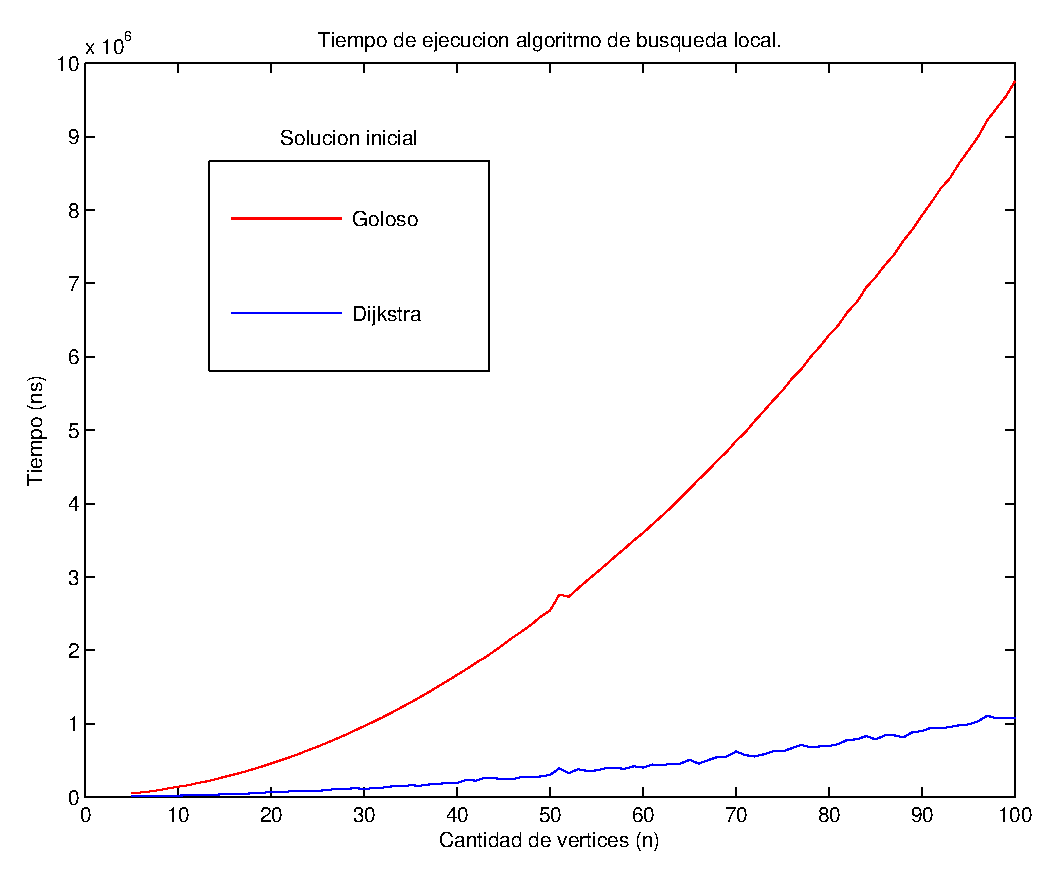
\includegraphics[width=\linewidth]{graficos/busq_local_tiempo.eps}
    \caption{Tiempo ejecución búsqueda local}\label{fig:busq-local-tiempo}
  \end{minipage}
  \hfill
  \begin{minipage}{0.5\linewidth}
    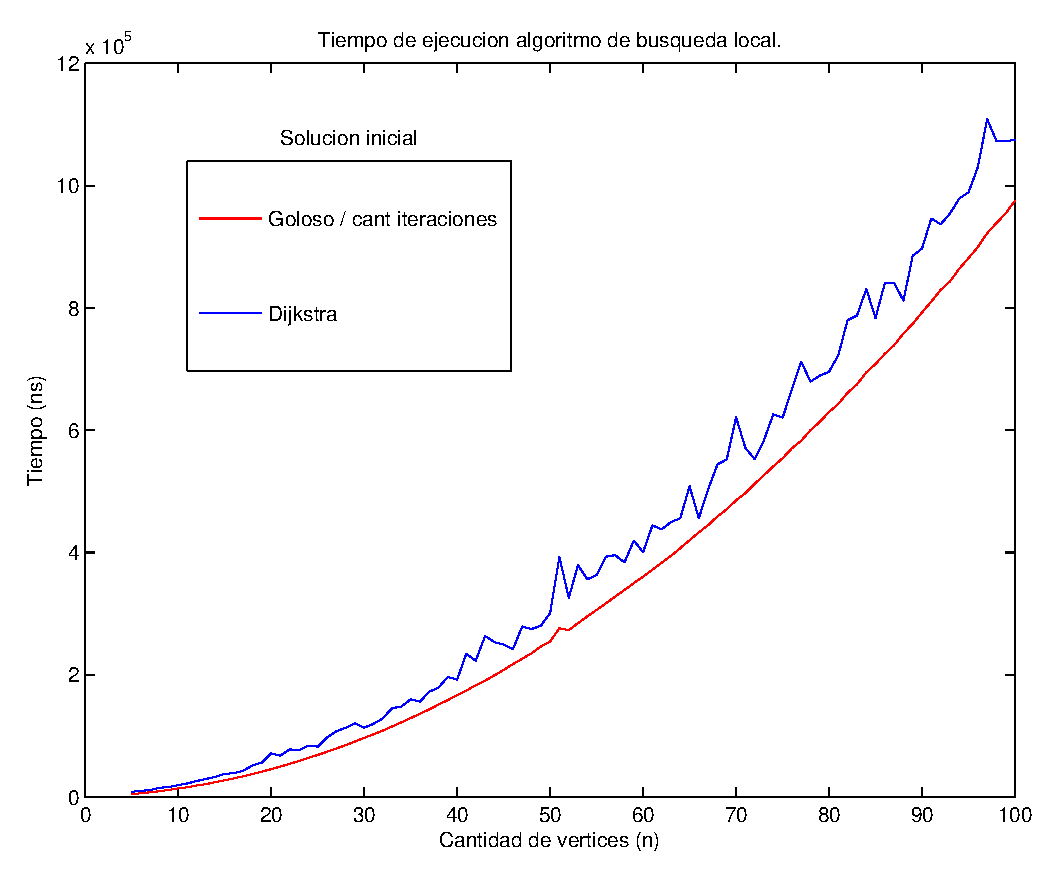
\includegraphics[width=\linewidth]{graficos/busq_local_tiempo_divido10.eps}
    \caption{Idem divido 10}\label{fig:busq-local-tiempo-div10}
  \end{minipage}
\end{figure}

Como podemos observar en el gráfico de la Figura \ref{fig:busq-local-tiempo} el algoritmo de búsqueda local utilizando nuestro algoritmo goloso tiene un tiempo de ejecución mayor al que utiliza el algoritmo de Dijkstra. Esto se debe a que lo que medimos es el tiempo en correr primero los algoritmos que generan las soluciones iniciales y luego correr el algoritmo de búsqueda local. Como ya sabemos nuestro algoritmo goloso corre el algoritmo de Dijkstra una cantidad de iteraciones prefijada. Resulta lógico pensar que un algoritmo que corre el algoritmo de Dijkstra muchas veces tendrá un tiempo de ejecución mayor al de un algoritmo que lo corre sólo una.

Por esto en el gráfico de a Figura \ref{fig:busq-local-tiempo-div10} mostramos los mismos tiempos que en el otro gráfico pero dividimos el tiempo que tarda el algoritmo de búsqueda local que usa nuestro algoritmo goloso por \emph{cant iteraciones}. Con este gráfico, logramos ver que el tiempo de ejecución de ambos algoritmos de búsqueda es parecido cuando reducimos el factor de tiempo de ejecución del algoritmo nos da la solución inicial.

A continuación incluimos unos gráficos que comparan la calidad de las soluciones del algoritmo de búsqueda local.

\begin{figure}[H]
  \begin{minipage}{0.5\linewidth}
    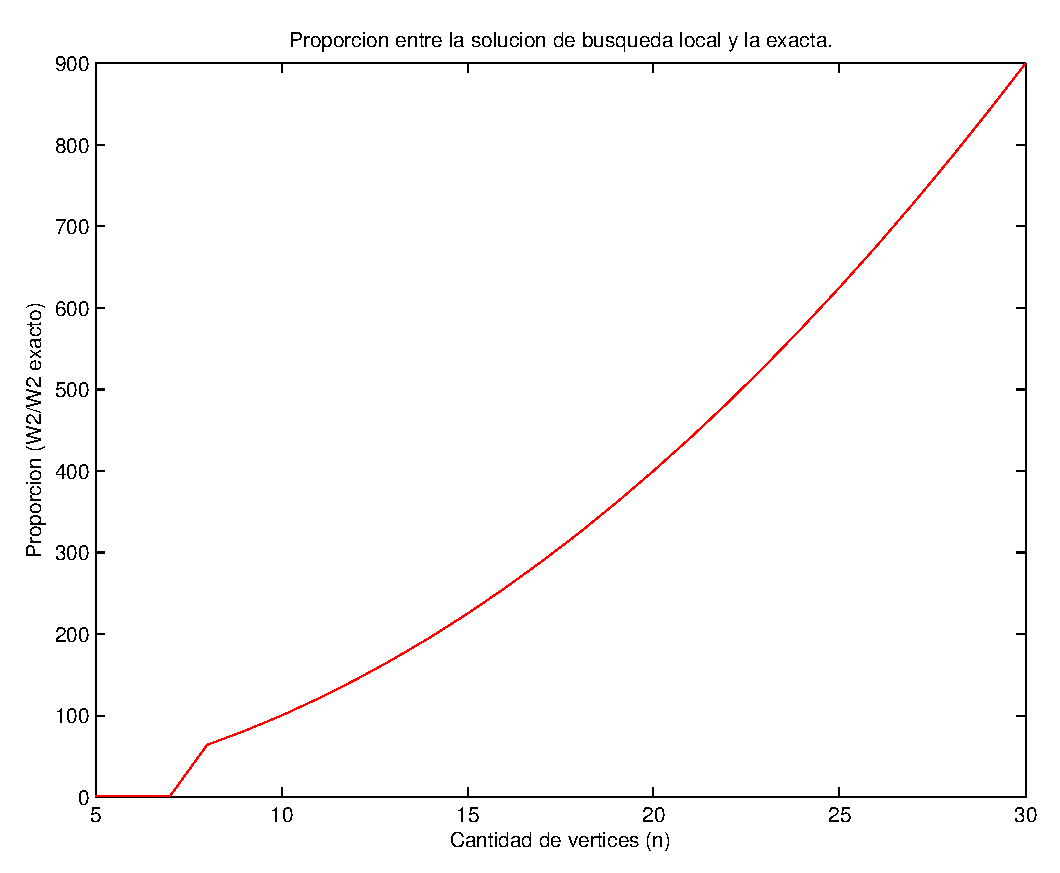
\includegraphics[width=\linewidth]{graficos/busq_local_proporcion.eps}
    \caption{Diferencia proporcional busqueda/exacto}\label{fig:busq-local-proporcion}
  \end{minipage}
  \hfill
  \begin{minipage}{0.5\linewidth}
    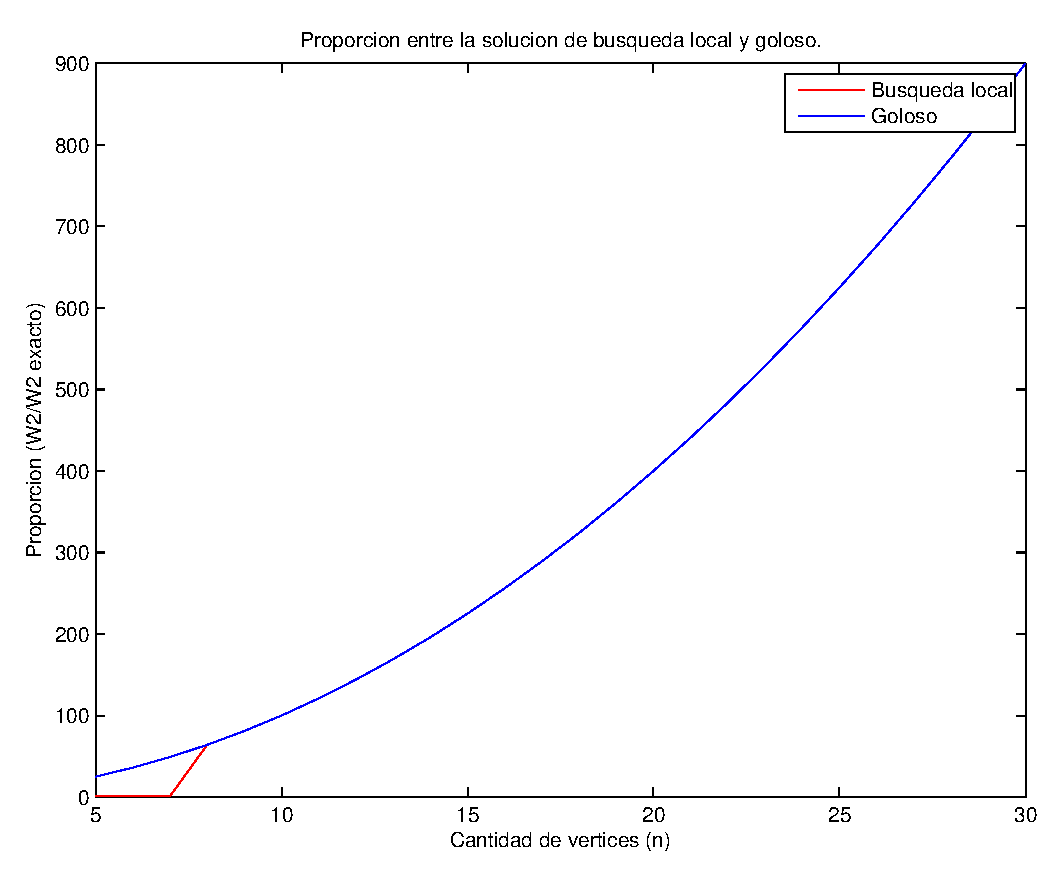
\includegraphics[width=\linewidth]{graficos/busq_local_proporcion_comparacion.eps}
    \caption{Calidad Soluciones Goloso/Dijkstra en familia \emph{3-caminos}}\label{fig:busq-local-proporcion-comparacion}
  \end{minipage}
\end{figure}

El gráfico de la Figura \ref{fig:busq-local-proporcion} muestra la diferencia proporcional entre las soluciones que nos da el algoritmo de búsqueda local con una solución inicial dada por nuestro algoritmo goloso y el algoritmo exacto para la familia de grafos que rompe nuestro algoritmo goloso \emph{3-caminos}. El gráfico de la Figura \ref{fig:busq-local-proporcion-comparacion} compara la proporción con respecto al algoritmo exacto de las soluciones dadas por el algoritmo goloso y las soluciones resultantes de aplicar búsqueda local tomando como soluciones iniciales a las soluciones dadas por el algoritmo goloso para la misma familia de grafos del gráfico de la Figura \ref{fig:busq-local-proporcion}. Mostramos esto en dos gráficos distintos para que se logre apreciar que para la mayoría de los casos, el algoritmo de búsqueda local no logra mejorar las soluciones del nuestro algoritmo goloso para esta familia.

Vale aclarar que en este experimento pudimos correr el algoritmo exacto para grafos con una cantidad de nodos un poco mayor que en las anteriores mediciones. Esto se debe a que para esta familia de grafos el algoritmo exacto tarda menos tiempo en correr ya que hay menos caminos que revisar (recordemos que los grafos de nuestra familia se componen de tres caminos disjuntos en aristas).

Como podemos observar para $n \leq 7$ el algoritmo de búsqueda local logra mejorar la calidad de la solución dada por el nuestro algoritmo goloso. Sin embargo, cuando $n > 7$ no logra mejorarla. Esto verifica lo que dijimos en la sección \ref{subsub:algoritmos-heuristicos-busqueda-calidad.tex}.

Para continuar experimentando, incluimos un gráfico que muestre como se comporta nuestro algoritmo de búsqueda local ante grafos que sean de la familia \emph{3-caminos con puentes} definida en la sección \ref{subsub:algoritmos-heuristicos-busqueda-calidad.tex}. 

\begin{figure}[H]
  \begin{center}
    \begin{minipage}{0.5\linewidth}
      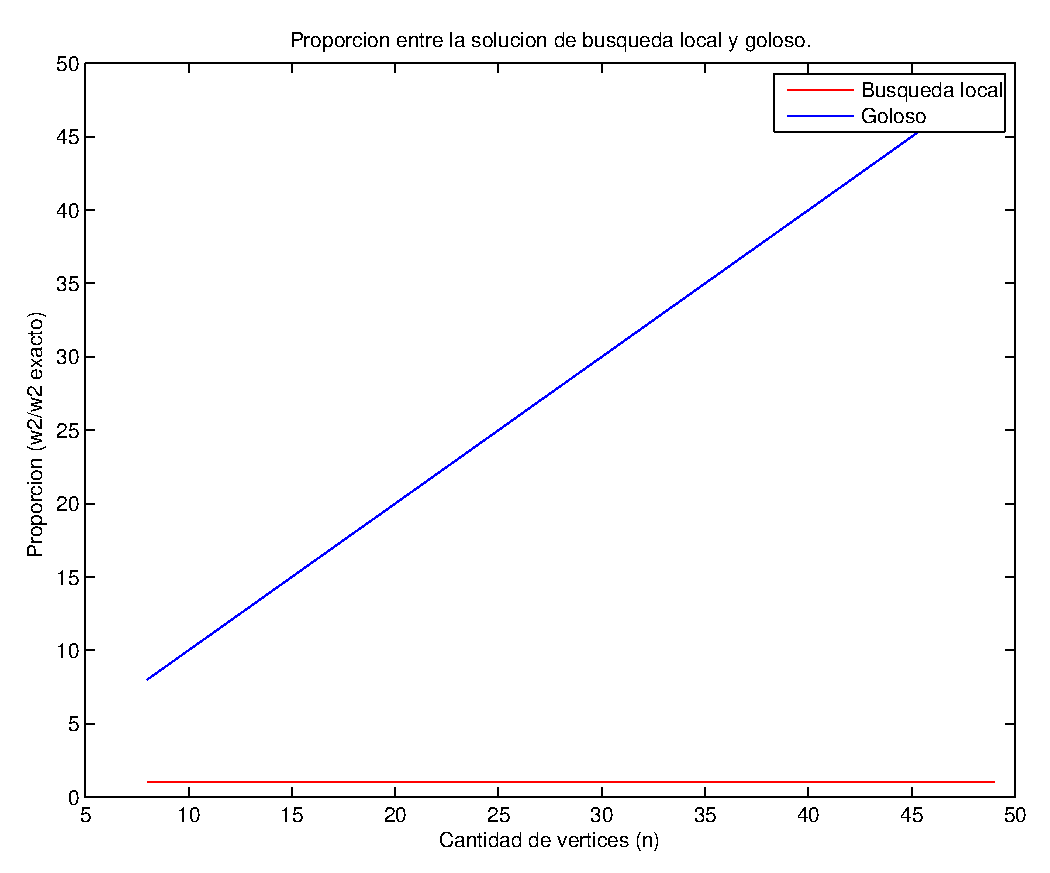
\includegraphics[width=\linewidth]{graficos/busq_local_proporcion2.eps}
      \caption{Calidad Soluciones Goloso/Dijkstra en familia \emph{3-caminos con puentes}}\label{fig:busq-local-proporcion-2}
    \end{minipage}
  \end{center}
\end{figure}

En el gráfico podemos observar el comportamiento del algoritmo de búsqueda local en proporción al algoritmo exacto comparado al comportamiento del algoritmo goloso, también en proporción. Como podemos observar en esta familia el algoritmo de búsqueda local sí puede mejorar la solución que el algoritmo goloso le da como inicial. Más aún, el grafico nos permite observar que no sólo las mejora, sino que logra encontrar la solución óptima, ya que como vemos el peso $W2$ de la solución dada por dicho algoritmo es igual al del de la solución del algoritmo exacto. Esto verifica lo que dijimos en la sección \ref{subsub:algoritmos-heuristicos-busqueda-calidad.tex}.

A continuación incluiremos un gráfico que compara la calidad de las soluciones del algoritmo de busqueda local cuando éste toma como solución inicial la dada por el algoritmo de Dijkstra tomando como función de peso el para las aristas la función $\omega_1$

\begin{figure}[H]
  \begin{center}
    \begin{minipage}{0.5\linewidth}
      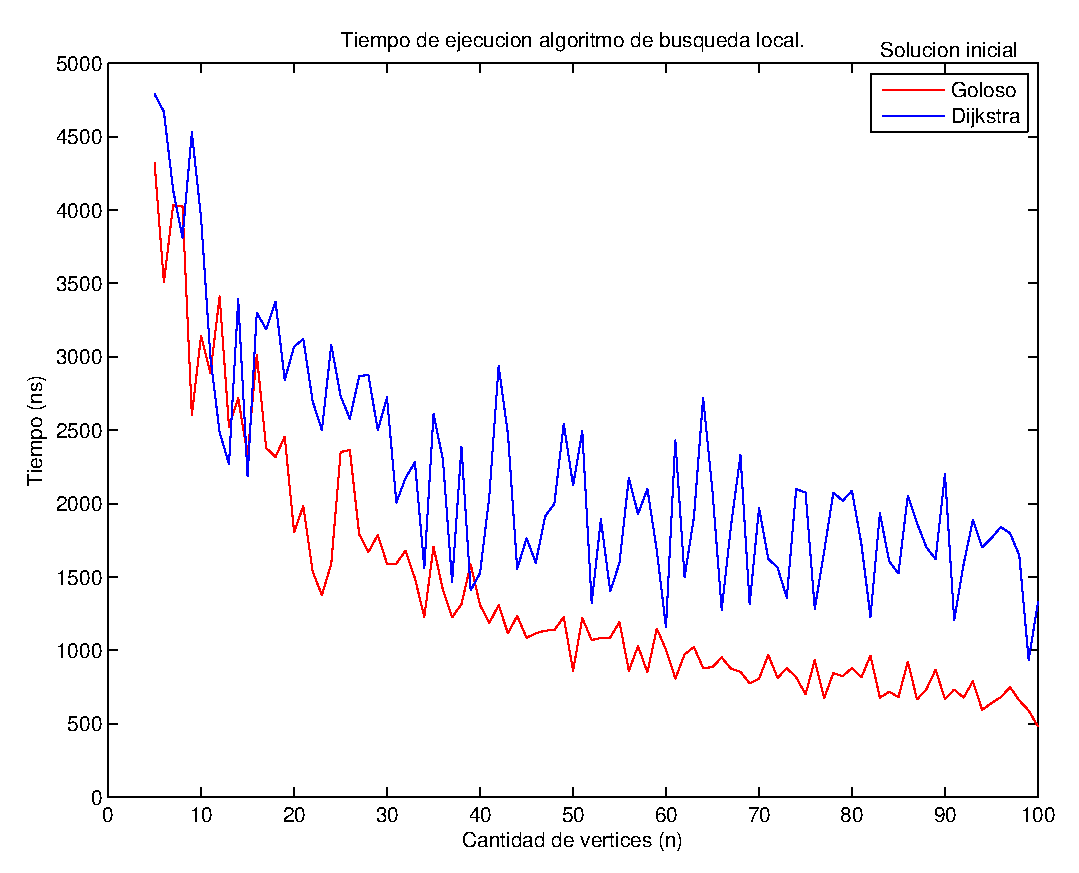
\includegraphics[width=\linewidth]{graficos/busq_local_calidad.eps}
      \caption{Comparacion Soluciones iniciales}\label{fig:busq-local-calidad}
    \end{minipage}
  \end{center}
\end{figure}
  
Como podemos observar en la Figura \ref{fig:busq-local-calidad}, para los grafos con los que hicimos las mediciones, el algoritmo que toma como solución inicial la dada por nuestro algoritmo goloso en general es mejor que la dada por el algoritmo de Dijkstra.

%TODO decir porque es mejor con el goloso
Creemos que esto es así porque, como ya vimos en la sección \ref{subsub:algoritmos-heuristicos-goloso-experimentacion.tex} las soluciones dadas por nuestro algoritmo goloso son mejores que las dadas por el algoritmo de Dijkstra. Una vez que nuestro algoritmo de búsqueda local toma estas soluciones iniciales mejora ambas. Sin embargo, no la logra mejorar lo suficiente las soluciones dadas por el algoritmo de Dijkstra como para que dichas soluciones superen a las dadas por nuestro algoritmo goloso, una vez que son mejoradas por búsqueda local.

Debido a los resultados obtenidos anteriormente, llegamos a la conclusión de que, en general, resulta mejor utilizar nuestro algoritmo goloso para generar las soluciones iniciales que utilizar el algoritmo de Dijkstra tomando $\omega_1$ como función de peso. Por lo tanto, a partir de ahora utilizaremos únicamente nuestro algoritmo goloso para generar las soluciones iniciales para luego aplicarles busqueda local.
  \newpage

  \subsection{Heuristica GRASP}
  \label{sub:algoritmos-heuristicos-grasp}
      \subsubsection{Desarrollo del algoritmo}
      \label{subsub:algoritmos-heuristicos-grasp-desarrollo.tex}
      En esta sección describiremos detalladamente el diseño de nuestro algoritmo de búsqueda local. 

\subsubsection{Vecindad}

La escencia de este algoritmo se encuentra principalmente en la vecindad que elegimos para las posibles soluciones, a continuación la detallaremos.

Supongamos que tenemos un camino $C$ = ($c_0$, $c_1$, ..., $c_k$) de $k+1$ nodos que es una solución factible del problema de CACM par un grafo $G$ = ($V$,$E$). Los vecinos de la solución $C$ son caminos que también sean soluciones factibles y que surgan de aplicarle una de las siguientes operaciones:

$\bullet$ Quitar Nodo:

Supongamos que existe un $i$ tal que $0 < i < k$ y que ($c_{i+1}$, $c_{i+1}$) $\in$ $E$. Bajo estas condiciones podemos afirmar que existe un camino en $G$ llamado $C'$ tal que $C'$ = ($c_0$, ..., $c_{i-1}$, $c_{i+1}$, ..., $c_k$). Esto significa que dado $C$ podemos eliminar el nodo $c_i$ del camino y unir $c_{i-1}$ y $c_{i+1}$ ya que estos son adyacentes entre sí, obteniendo un camino $C'$ de $k$ nodos.

$\bullet$ Agregar Nodo:

La operación agregar nodo es la operación inversa a la operación Quitar Nodo descripta anteriormente. Supongamos que existe un $i$ tal que $0 \leq i < k$ y existe un nodo $w \in V$ tal que ($c_i$,$w$) $\in E$ y ($w$, $c_{i+1}$) $\in E$. En este caso podemos afirmar que podemos construir un camino $C'$ = ($c_0$, ..., $c_{i}$,$w$,$c_{i+1}$) de $k+2$ nodos.

Vale aclarar que para realizar esta operación, el nodo $w$ no debe pertenecer a $C$, ya que queremos que el camino sea simple.

$\bullet$ Cambiar Nodo:

Esta operación es una mezcla de las dos operaciones anteriores. Supongamos que existe un $i$ tal que $0 \leq i < k-1$ y que existe un nodo $w \in V$ (nuevamente, $w$ no debe estar en el camino $C$) tal que ($c_i$,$w$) $\in E$ y ($w$, $c_{i+2}$) $\in E$. En este caso podemos cambiar el nodo $c_{i+1}$ del camino $C$ por el nodo $w$ obteniendo un nuevo camino $C'$ de la misma cantidad de nodos.

Uno podría creer que la operación Cambiar Nodo es una combinación de las dos operaciones descriptas anteriormente Agregar Nodo y Quitar Nodo, ya que se podría quitar primero el nodo $c_{i+1}$ y luego agregar el nodo $w$. Sin embargo, esto no es así ya que podría pasar que el eje ($c_i$,$c_{i+2}$) $\notin E$ y, si esto ocurre no nos sería posible quitar el nodo $c_{i+1}$ para luego agregar el nodo $w$.

Dadas estas tres operaciones, un vecino de una solución factible $C$ es un camino que se pueda construir aplicándole a $C$ una de estas tres operaciones. Nótese que si existiese un $C'$ que se pudiera construir a partir de aplicarle a $C$ más de una operación, $C'$ no sería vecino de $C$. Tomamos esta decisión debido a que pensamos que si consideráramos vecino a un camino que se pudiera construir a partir de aplicarle numerosas operaciones a $C$ se estaría perdiendo, por así decirlo, la localidad de la búsqueda y estaríamos incurriendo en una búsqueda más global. Es importante recalcar que sólo tomamos como un vecino de $C$ un camino $C'$ factible.

Algo que pensamos mientras elegíamos nuestra vecindad es que una buena propiedad que ésta pudiese cumplir sería que, dada una solución factible $C$, aplicándole una cantidad de operaciones, pudiésemos llegar a cualquier otra solución factible.

Para explicar esto pensemos en los números reales. Supongamos tenemos una función $F: \mathbb{R} \Rightarrow \mathbb{R}$ y queremos hallar su máximo mediante una búsqueda local. Para esto podemos elegir, dado un $c \in \mathbb{R}$, una función de vecindad que devuelva por ejemplo el conjunto $[c-\varepsilon, c+\varepsilon]$  para algún $\varepsilon$. Dada esta función de vecindad podemos observar que aplicándola muchas veces nos podemos mover a lo largo de todo el dominio de la función $F$.

Que una función de vecindad cumpla con esta propiedad nos parece bueno porque al poder moverse de cualquier solución factible a cualquier otra, nos garantizamos de que no habrá soluciones factibles buenas que nos estemos perdiendo. Más aún, si esta propiedad vale podemos afirmar que si aplicamos muchas veces la función de vecindad (empezando de una solución $C$ luego en un vecino de $C$ y así) eventualmente podemos llegar a la solución óptima del problema (aunque probablemente sea necesario aplicar esta función un número inmenso de veces para llegar y no se estaría haciendo búsqueda local).

Luego de pensarlo llegamos a la conclusión de que nuestra vecindad no cumple con esa propiedad, ya que existen casos en los que a partir de una solución nos es imposible llegar a otra.

Supongamos que nuestro grafo es $C_n$ y que nuestro nodo inicial es $c_1$ y nuestro nodo destino es $c_n$. Supongamos además que tenemos una solución que es $S$ = ($c_1$, $c_2$, ... , $c_n$). Podemos observar que hay otra posible solución, que es $S'$ = ($c_1$,$c_n$) ya que como nuestro grafo es $C_n$ entonces $c_1$ y $c_n$ están unidos. Sin embargo, con nuestra función de vecindad nos es imposible llegar de la solución $S$ a la solución $S'$. ya que no hay ninguna operación que se pueda realizar a $S$. 

Supongamos ahora que tenemos como solución inicial $S'$. En este caso tampoco podemos aplicar ninguna operación a $S'$ y no podremos llegar a la otra solución. Podemos decir que en este caso, en nuestra vecindad tanto $S$ como $S'$ son soluciones sin vecinos.

Luego de pensar como solucionar este problema, llegamos a la conclusión de que para resolverlo deberíamos tener una vecindad muy grande y perderíamos la localidad de la búsqueda. Por ejemplo, en el caso anterior, para llegar de la solución $S'$ a la solución $S$ una operación debería ser agregar a $S'$ un camino de $n$ nodos, lo cual es fácil para el grafo $C_n$ pero muy complejo para otros grafos.

\subsubsection{Algoritmo}

Habiendo explicado las características de nuestra vecindad, a continuación describiremos el algoritmo de busqueda local.

Nuestro algoritmo recibe como entrada el grafo $G$ y una solución inicial $C$. Luego de esto el algoritmo entra en un ciclo en el que se buscan los vecinos de la mejor solución $S$ que se tenga. Si existe un vecino $S'$ mejor que $S$, entonces la mejor solución pasa a ser $S'$ y pasamos a la siguiente iteración. En la iteración en la que no exista un vecino mejor que $S$ entonces se termina la búsqueda.
%TODO: En realidad búsqueda local siempre es así, deberíamos sacar este párrafo?

A continuación incluiremos un pseudocódigo del algoritmo.
\begin{center}
 \begin{figure}[H]
  \begin{pseudo}
   \Procedure{busqueda local}{grafo G, camino sol}
   \State $mejorSol \leftarrow sol$
   \While{$seguirBuscando$}
      \State $buscarVecinoQuitar(mejorSol, mejorVecino, G)$
      \State $buscarVecinoAgregar(mejorSol, mejorVecino, G)$
      \State $buscarVecinoCambiar(mejorSol, mejorVecino, G)$
      \If{$mejorVecino.W_1 > k \vee mejorVecino.W_1 \geq mejorSol.W_1$}
	\State $seguirBuscando \leftarrow false$
      \Else
	\State $actualizar(mejorSol, mejorVecino)$
      \EndIf
      \State Devolver $mejorSol$
   \EndWhile
   \EndProcedure
  \end{pseudo}
 \end{figure}
\end{center}

En este algoritmo usamos la estructura Camino, que es una lista de ejes y además tiene el peso total $W_1$ y $W_2$. Y además usamos la estructura vecino, que tiene tres tipos: $TIPO1$ significa que es un vecino que surge de eliminar un nodo de la solución actual, $TIPO2$ que surge de agregar un nodo, o $TIPO3$, que surge de cambiar un nodo por otro. Además la estructura tiene una posición donde hay que hacer los cambios para pasar del camino actual al vecino (estos cambios se deducen según el tipo del vecino que sea). Por último la estructura cuenta con una lista de nodos a agregar al camino actual, si se cambia o agrega un nodo la lista tendrá un elemento y si se elimina un nodo la lista será vacía.

Utilizamos esta estructura para poder pasar de un camino a su vecino en una complejidad constante ya que ésta cuenta con la información necesaria para saber cuáles son los cambios a realizar y dónde hay que realizarlos. Si no contáramos con esta estructura y tuviésemos simplemente otro camino deberíamos copiar el camino para actualizar la solución, lo que tendría una complejidad temporal lineal.

      \subsubsection{Complejidad temporal de peor caso}
      \label{subsub:algoritmos-heuristicos-grasp-complejidad.tex}
      \begin{center}
 \begin{figure}[H]
  \begin{pseudo}
   \Procedure{cacm\_goloso}{grafo $G$, nodo $u$, nodo $v$}
    \State $pInicial \leftarrow 0$, $pFinal \leftarrow 1$, $pMedio$ \Ode{1}
    \For{$i < Cant\_Iteraciones$}
      \State $pMedio \leftarrow (pInicial + pFinal)/2$ \Ode{1}
      \State $solucion$ $\leftarrow$ $Dijkstra(G$, $pMedio$, $u$, $v)$ \Ode{n^2}
      \If{$W_1(solucion) \leq k$} \Ode{1}
	 \State $pInicial \leftarrow pMedio$ \Ode{1}
      \Else
	 \State $pFinal \leftarrow pMedio$ \Ode{1}
      \EndIf
    \EndFor
    \If{$W_1(solucion) \leq k$} \Ode{1}
      \State $solucion \leftarrow Dijkstra(G, 1)$ \Ode{n^2}
    \EndIf
    \State Devolver solución \Ode{1}
   \EndProcedure
  \end{pseudo}
 \end{figure}
\end{center}

 Como podemos ver el algoritmo esta compuesto por una instrucción $O(1)$ luego un for,y por ultimo 2 $O(1)$ y una vez Dijkstra, que como sabemos tiene complejidad $O(n^2)$. El for itera $Cant\_Iteraciones$ instrucciones $4*O(1) + O(n^2)$. Como $Cant\_Iteraciones$ es un numero acotado, la complejidad del for es $O(n^2)$. Por álgebra de ordenes $O(1)+O(n^2)+2*O(1)+O(n^2)=O(n^2)$.  

      \subsubsection{Experimentación}
      \label{subsub:algoritmos-heuristicos-grasp-experimentacion.tex}
      En esta sección, realizaremos diversos experimentos para verificar tanto el tiempo de ejecución como la calidad de las soluciones de nuestro algoritmo de búsqueda local.

Como dijimos anteriormente, el algoritmo de búsqueda local toma una solución inicial. Nosotros tomamos como un parámetro del algoritmo la solución inicial que éste recibe.

En los gráficos que presentamos a continuación, mostramos el tiempo de ejecución de correr búsqueda local con dos algoritmos que nos dan soluciones iniciales. Un algoritmo es el algoritmo goloso que detallamos en la sección \ref{subsub:algoritmos-heuristicos-goloso-desarrollo.tex}, y el otro es el algoritmo de Dijkstra tomando como pesos de las aristas la función $\omega_1$.

\begin{figure}[H]
  \begin{minipage}{0.5\linewidth}
    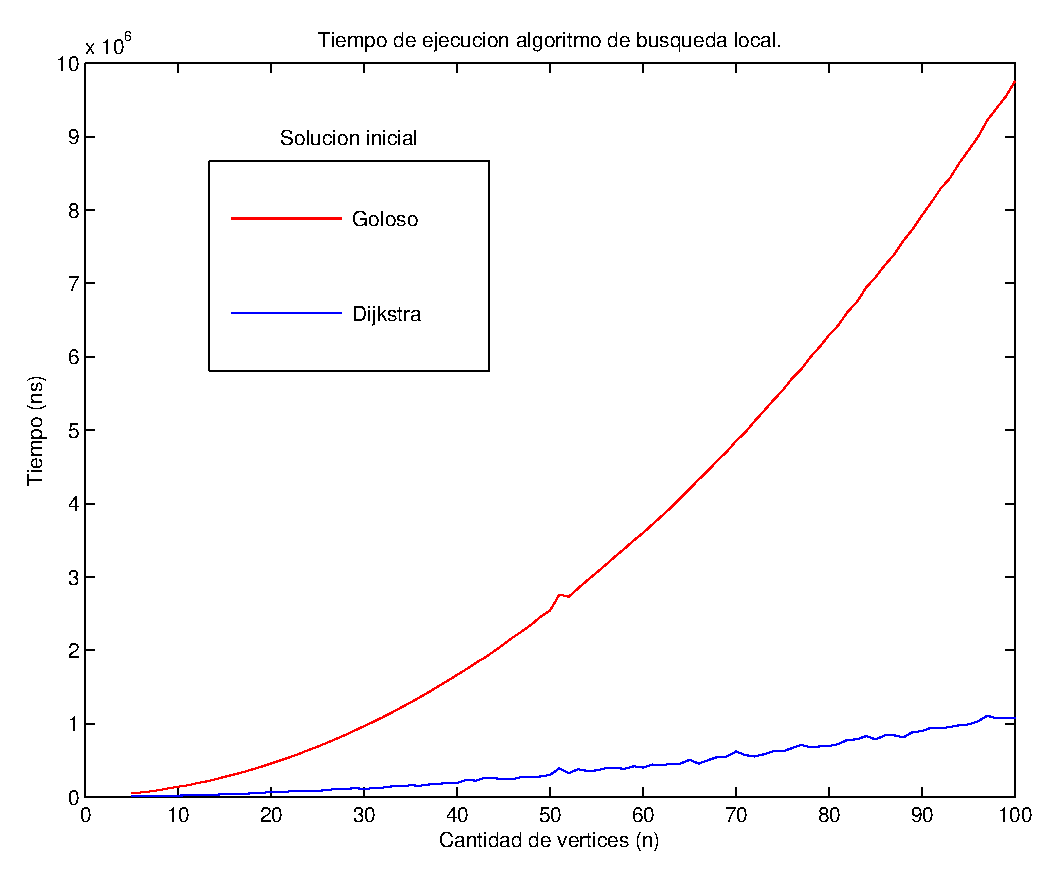
\includegraphics[width=\linewidth]{graficos/busq_local_tiempo.eps}
    \caption{Tiempo ejecución búsqueda local}\label{fig:busq-local-tiempo}
  \end{minipage}
  \hfill
  \begin{minipage}{0.5\linewidth}
    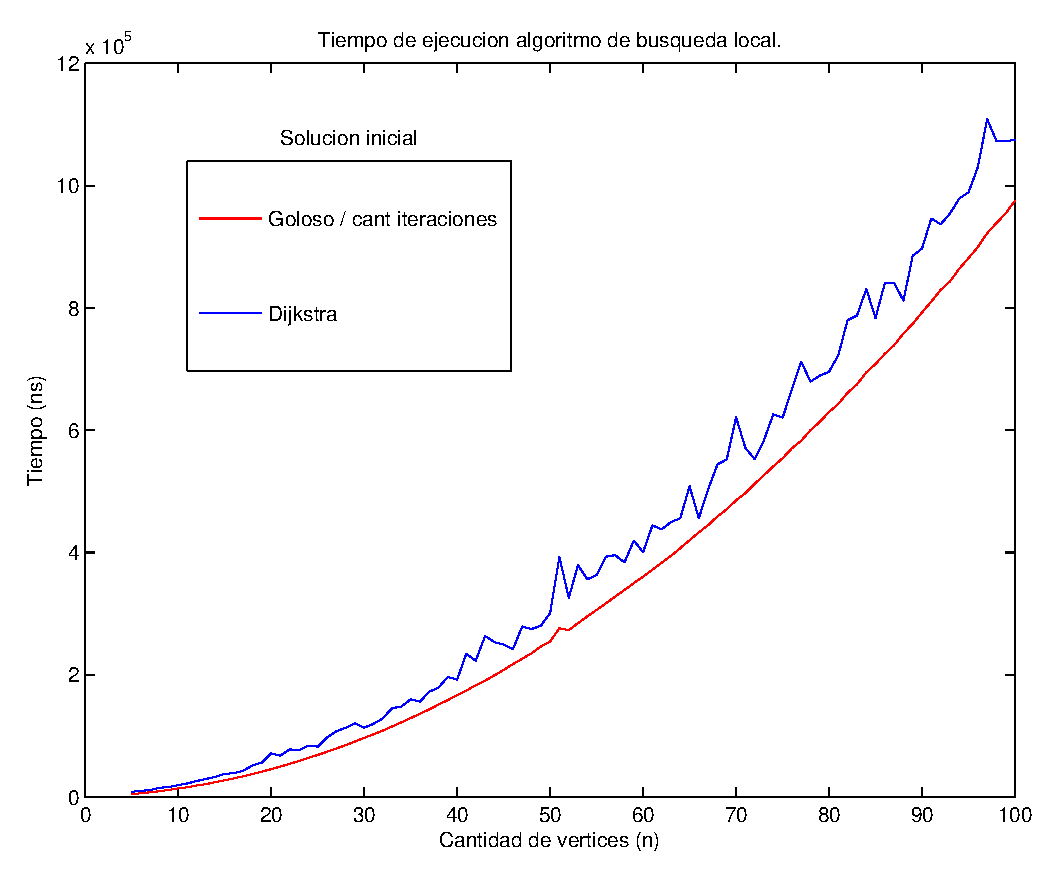
\includegraphics[width=\linewidth]{graficos/busq_local_tiempo_divido10.eps}
    \caption{Idem divido 10}\label{fig:busq-local-tiempo-div10}
  \end{minipage}
\end{figure}

Como podemos observar en el gráfico de la Figura \ref{fig:busq-local-tiempo} el algoritmo de búsqueda local utilizando nuestro algoritmo goloso tiene un tiempo de ejecución mayor al que utiliza el algoritmo de Dijkstra. Esto se debe a que lo que medimos es el tiempo en correr primero los algoritmos que generan las soluciones iniciales y luego correr el algoritmo de búsqueda local. Como ya sabemos nuestro algoritmo goloso corre el algoritmo de Dijkstra una cantidad de iteraciones prefijada. Resulta lógico pensar que un algoritmo que corre el algoritmo de Dijkstra muchas veces tendrá un tiempo de ejecución mayor al de un algoritmo que lo corre sólo una.

Por esto en el gráfico de a Figura \ref{fig:busq-local-tiempo-div10} mostramos los mismos tiempos que en el otro gráfico pero dividimos el tiempo que tarda el algoritmo de búsqueda local que usa nuestro algoritmo goloso por \emph{cant iteraciones}. Con este gráfico, logramos ver que el tiempo de ejecución de ambos algoritmos de búsqueda es parecido cuando reducimos el factor de tiempo de ejecución del algoritmo nos da la solución inicial.

A continuación incluimos unos gráficos que comparan la calidad de las soluciones del algoritmo de búsqueda local.

\begin{figure}[H]
  \begin{minipage}{0.5\linewidth}
    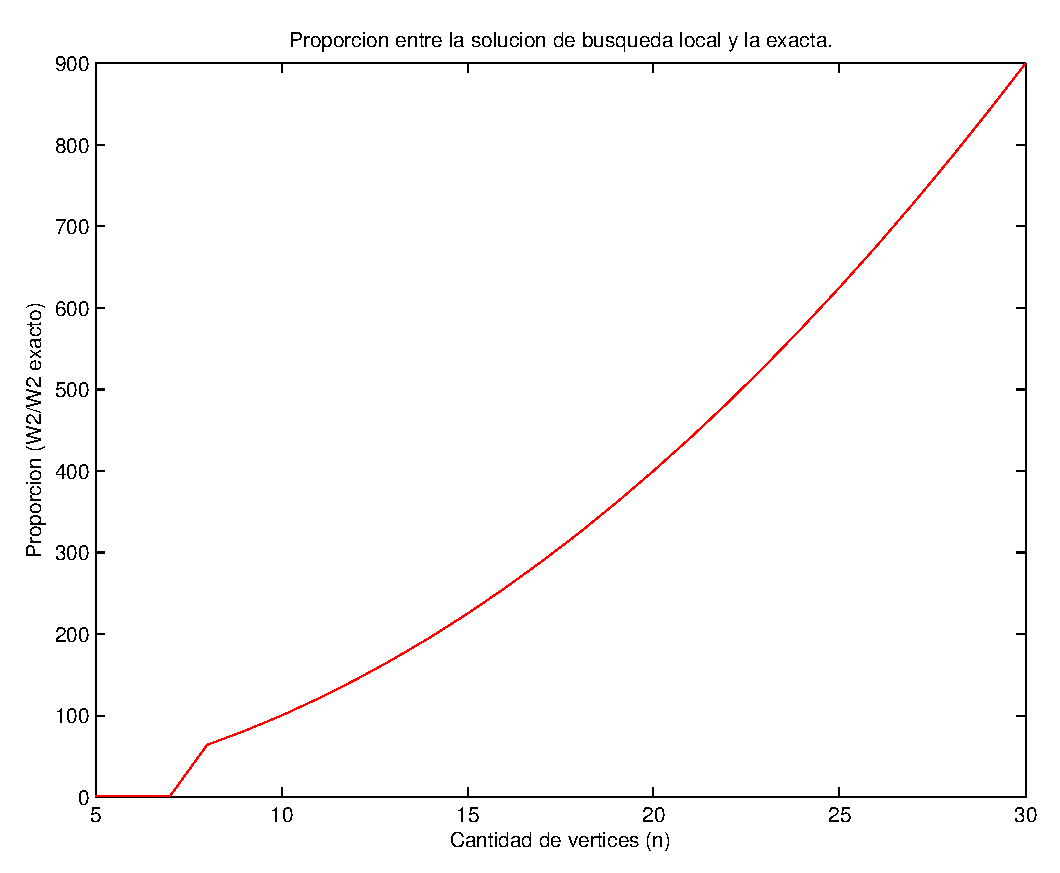
\includegraphics[width=\linewidth]{graficos/busq_local_proporcion.eps}
    \caption{Diferencia proporcional busqueda/exacto}\label{fig:busq-local-proporcion}
  \end{minipage}
  \hfill
  \begin{minipage}{0.5\linewidth}
    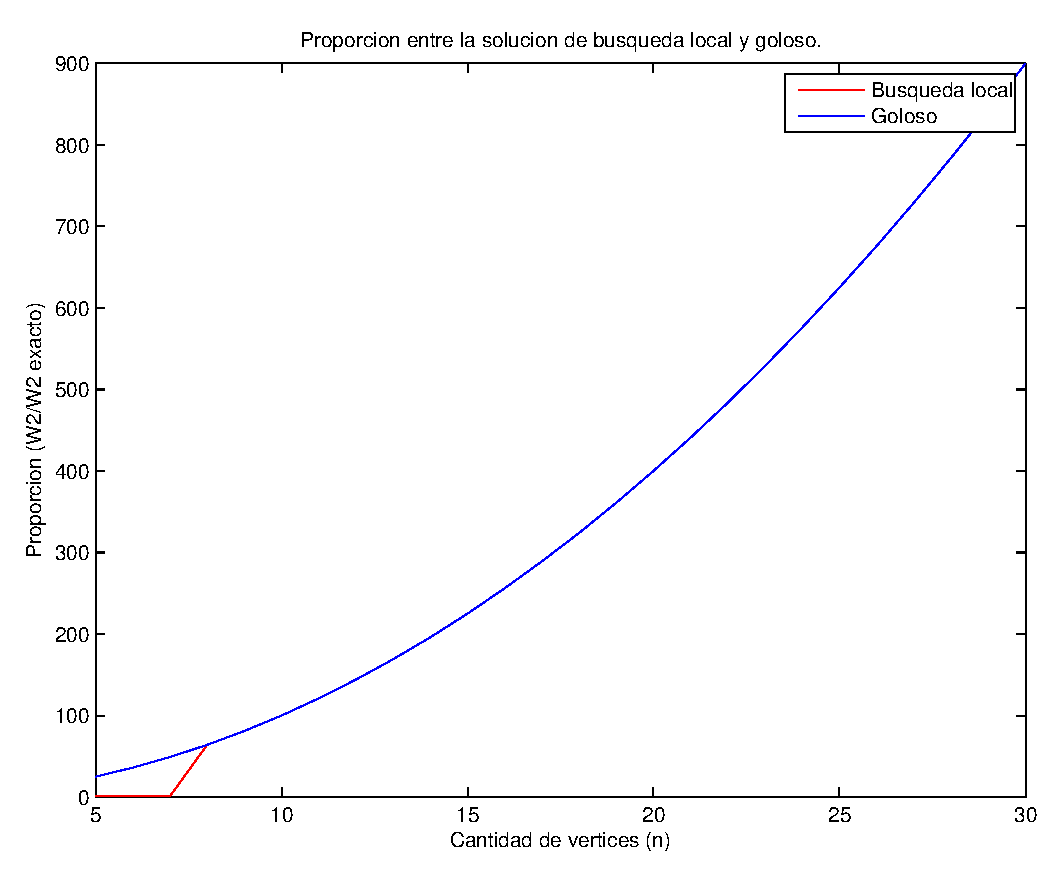
\includegraphics[width=\linewidth]{graficos/busq_local_proporcion_comparacion.eps}
    \caption{Calidad Soluciones Goloso/Dijkstra en familia \emph{3-caminos}}\label{fig:busq-local-proporcion-comparacion}
  \end{minipage}
\end{figure}

El gráfico de la Figura \ref{fig:busq-local-proporcion} muestra la diferencia proporcional entre las soluciones que nos da el algoritmo de búsqueda local con una solución inicial dada por nuestro algoritmo goloso y el algoritmo exacto para la familia de grafos que rompe nuestro algoritmo goloso \emph{3-caminos}. El gráfico de la Figura \ref{fig:busq-local-proporcion-comparacion} compara la proporción con respecto al algoritmo exacto de las soluciones dadas por el algoritmo goloso y las soluciones resultantes de aplicar búsqueda local tomando como soluciones iniciales a las soluciones dadas por el algoritmo goloso para la misma familia de grafos del gráfico de la Figura \ref{fig:busq-local-proporcion}. Mostramos esto en dos gráficos distintos para que se logre apreciar que para la mayoría de los casos, el algoritmo de búsqueda local no logra mejorar las soluciones del nuestro algoritmo goloso para esta familia.

Vale aclarar que en este experimento pudimos correr el algoritmo exacto para grafos con una cantidad de nodos un poco mayor que en las anteriores mediciones. Esto se debe a que para esta familia de grafos el algoritmo exacto tarda menos tiempo en correr ya que hay menos caminos que revisar (recordemos que los grafos de nuestra familia se componen de tres caminos disjuntos en aristas).

Como podemos observar para $n \leq 7$ el algoritmo de búsqueda local logra mejorar la calidad de la solución dada por el nuestro algoritmo goloso. Sin embargo, cuando $n > 7$ no logra mejorarla. Esto verifica lo que dijimos en la sección \ref{subsub:algoritmos-heuristicos-busqueda-calidad.tex}.

Para continuar experimentando, incluimos un gráfico que muestre como se comporta nuestro algoritmo de búsqueda local ante grafos que sean de la familia \emph{3-caminos con puentes} definida en la sección \ref{subsub:algoritmos-heuristicos-busqueda-calidad.tex}. 

\begin{figure}[H]
  \begin{center}
    \begin{minipage}{0.5\linewidth}
      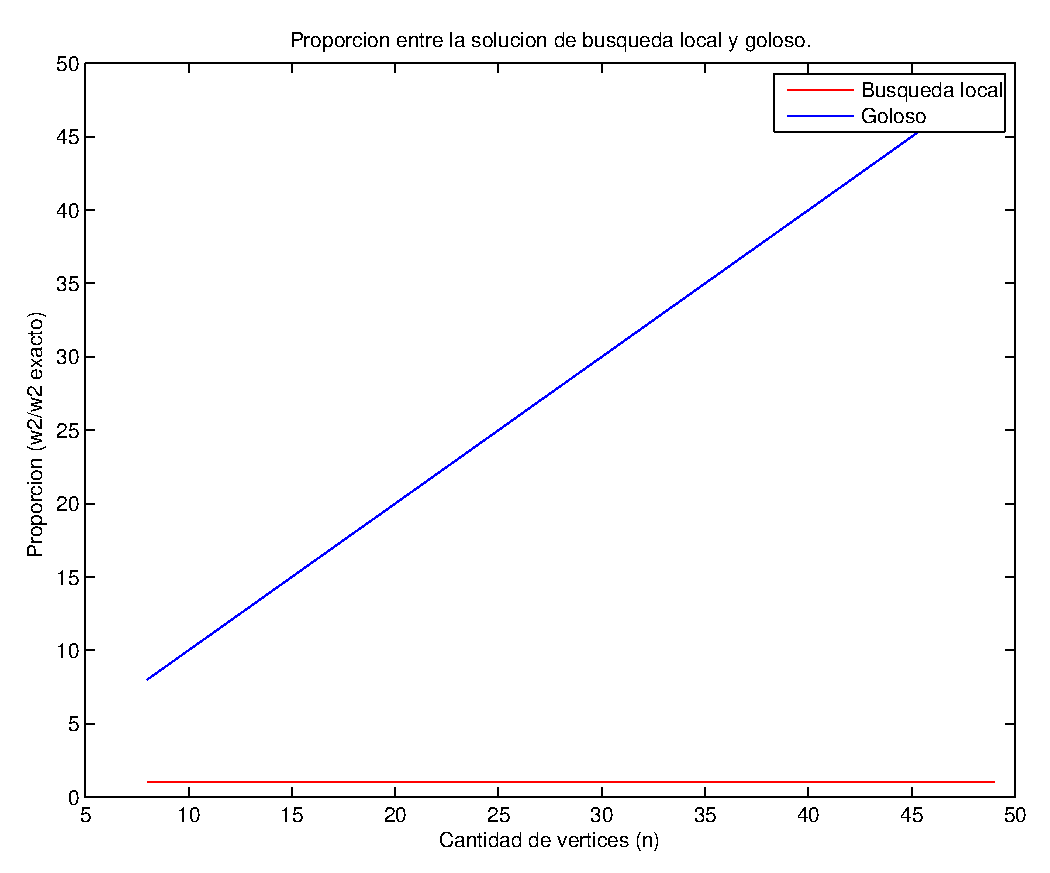
\includegraphics[width=\linewidth]{graficos/busq_local_proporcion2.eps}
      \caption{Calidad Soluciones Goloso/Dijkstra en familia \emph{3-caminos con puentes}}\label{fig:busq-local-proporcion-2}
    \end{minipage}
  \end{center}
\end{figure}

En el gráfico podemos observar el comportamiento del algoritmo de búsqueda local en proporción al algoritmo exacto comparado al comportamiento del algoritmo goloso, también en proporción. Como podemos observar en esta familia el algoritmo de búsqueda local sí puede mejorar la solución que el algoritmo goloso le da como inicial. Más aún, el grafico nos permite observar que no sólo las mejora, sino que logra encontrar la solución óptima, ya que como vemos el peso $W2$ de la solución dada por dicho algoritmo es igual al del de la solución del algoritmo exacto. Esto verifica lo que dijimos en la sección \ref{subsub:algoritmos-heuristicos-busqueda-calidad.tex}.

A continuación incluiremos un gráfico que compara la calidad de las soluciones del algoritmo de busqueda local cuando éste toma como solución inicial la dada por el algoritmo de Dijkstra tomando como función de peso el para las aristas la función $\omega_1$

\begin{figure}[H]
  \begin{center}
    \begin{minipage}{0.5\linewidth}
      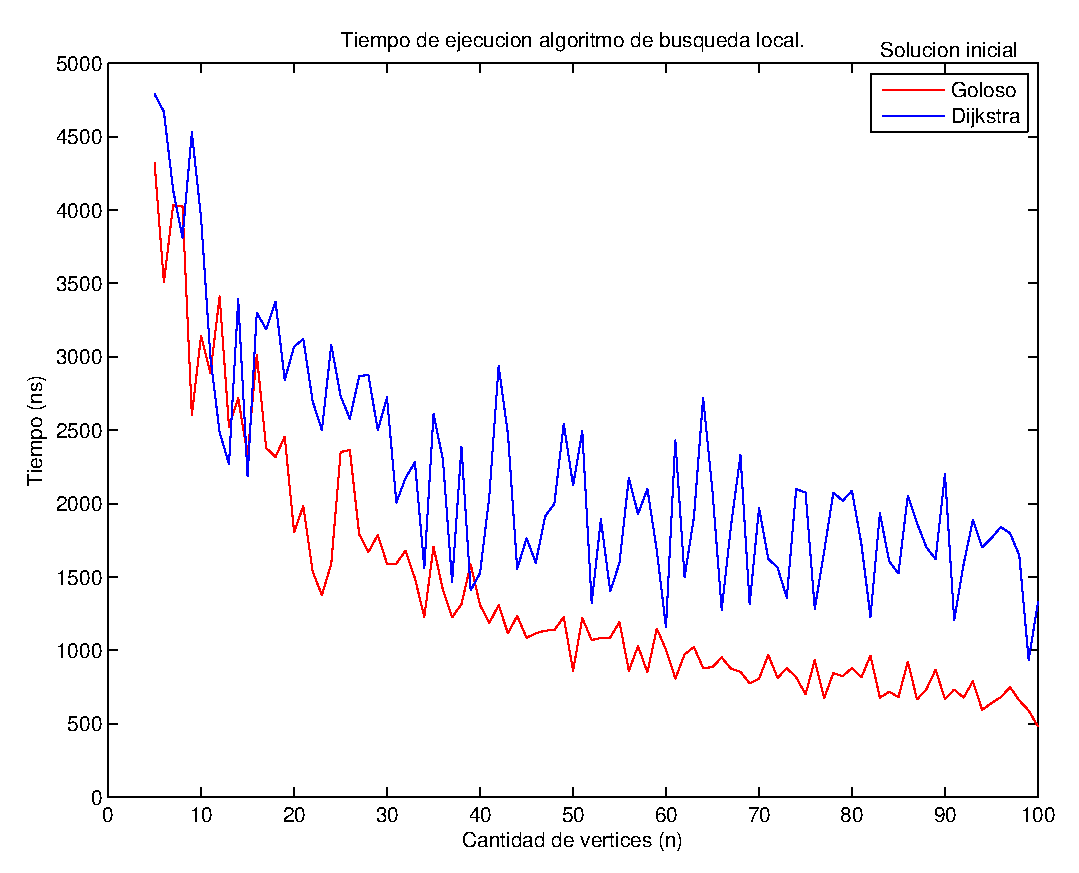
\includegraphics[width=\linewidth]{graficos/busq_local_calidad.eps}
      \caption{Comparacion Soluciones iniciales}\label{fig:busq-local-calidad}
    \end{minipage}
  \end{center}
\end{figure}
  
Como podemos observar en la Figura \ref{fig:busq-local-calidad}, para los grafos con los que hicimos las mediciones, el algoritmo que toma como solución inicial la dada por nuestro algoritmo goloso en general es mejor que la dada por el algoritmo de Dijkstra.

%TODO decir porque es mejor con el goloso
Creemos que esto es así porque, como ya vimos en la sección \ref{subsub:algoritmos-heuristicos-goloso-experimentacion.tex} las soluciones dadas por nuestro algoritmo goloso son mejores que las dadas por el algoritmo de Dijkstra. Una vez que nuestro algoritmo de búsqueda local toma estas soluciones iniciales mejora ambas. Sin embargo, no la logra mejorar lo suficiente las soluciones dadas por el algoritmo de Dijkstra como para que dichas soluciones superen a las dadas por nuestro algoritmo goloso, una vez que son mejoradas por búsqueda local.

Debido a los resultados obtenidos anteriormente, llegamos a la conclusión de que, en general, resulta mejor utilizar nuestro algoritmo goloso para generar las soluciones iniciales que utilizar el algoritmo de Dijkstra tomando $\omega_1$ como función de peso. Por lo tanto, a partir de ahora utilizaremos únicamente nuestro algoritmo goloso para generar las soluciones iniciales para luego aplicarles busqueda local.

\newpage


%%%%%%%%%%%%%%%%%%%%%%%%%%%%%%%%%%%%%%%%%%%%%%%%%%%%%%%%%%%%%%%%%%%%%%%%%%%%%%%
%% Comparación entre algoritmos y experimentación general                    %%
%%%%%%%%%%%%%%%%%%%%%%%%%%%%%%%%%%%%%%%%%%%%%%%%%%%%%%%%%%%%%%%%%%%%%%%%%%%%%%%

\section{Comparación entre algoritmos y experimentación general}
\label{sec:experimentacion-general}
En esta sección el objetivo será comparar todos los algoritmos diseñados e implementados en este trabajo.

A continuación incluiremos dos gráficos. Uno para poder observar como se comportan tanto nuestros algoritmos ante la familia de grafos \emph{3-caminos} y otro ante la familia \emph{3-caminos con puentes}.

\begin{figure}[H]
    \begin{minipage}{0.5\linewidth}
      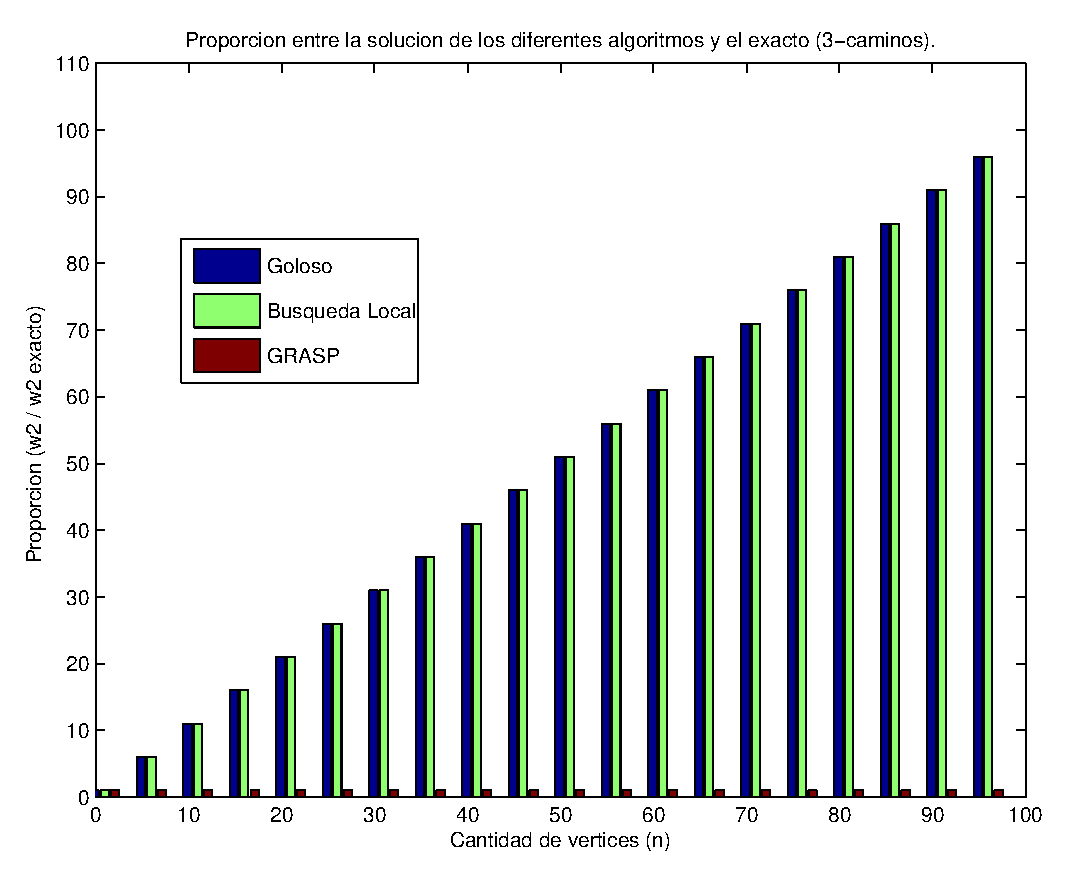
\includegraphics[width=\linewidth]{graficos/todos_proporcion_3caminos.eps}
      \caption{Comportamiento ante familia \emph{3-caminos}}\label{fig:comportamiento-familia-rompe}
    \end{minipage}
    \hfill
    \begin{minipage}{0.5\linewidth}
      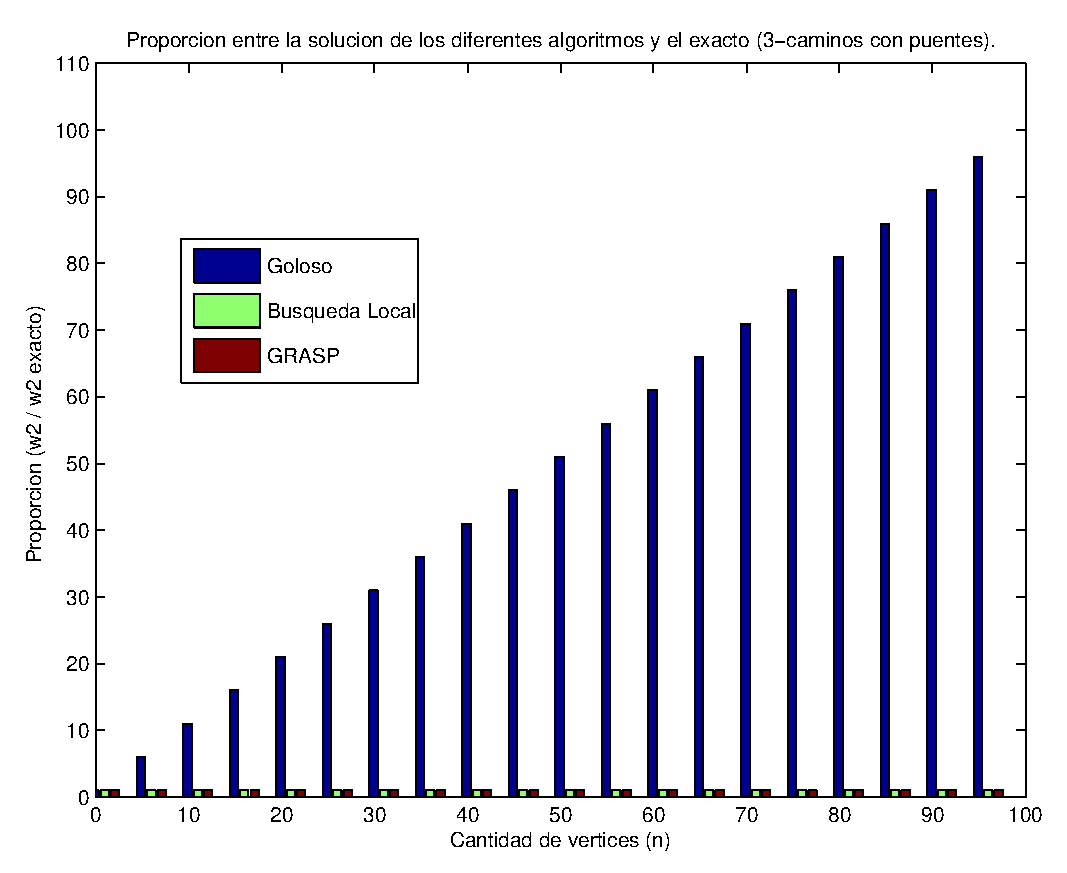
\includegraphics[width=\linewidth]{graficos/todos_proporcion_puentes.eps}
      \caption{Ídem familia \emph{3-caminos con puentes}}\label{fig:comportamiento-familia-puente}
    \end{minipage}    
\end{figure}

En estos gráficos mostramos el comportamiento de tanto de los siguientes algoritmos para dos familias de grafos. Los algoritmos medidos son los siguientes (todos en proporción al algoritmo exacto):

\begin{itemize}
 \item Algoritmo Goloso implementado en el trabajo
 \item Algoritmo de búsqueda local con algoritmo goloso como semilla
 \item Algoritmo GRASP que utiliza nuestro algoritmo goloso aleatorio y nuestro algoritmo de búsqueda local
\end{itemize}

Vale aclarar que todas las soluciones se muestran en proporción a las del algoritmo exacto.

En el gráfico de la Figura \ref{fig:comportamiento-familia-rompe} podemos ver que para los grafos de la familia \emph{3-caminos} nuestro algoritmo goloso devuelve soluciones de mala calidad, al igual que nuestro algoritmo de búsqueda local. Sin embargo, nuestro algoritmo GRASP logra mejorar las soluciones de dichos algoritmos. Más aún, no solo las mejora sino que devuelve la solución óptima. También podemos volver a ver que nuestro algoritmo de búsqueda local no logra mejorar la solución inicial que le da el algoritmo goloso para esta familia de grafos cuando éstos superan una determinada cantidad de nodos (en secciones previas observamos que dicha cantidad es $7$).

A su vez, en el gráfico de la Figura \ref{fig:comportamiento-familia-puente} podemos observar que nuestro algoritmo goloso devuelve malas soluciones para la familia de grafos \emph{3-caminos con puentes}, pero que el algoritmo de búsqueda local las logra mejorar, devolviendo una solución óptima. También podemos ver que el algoritmo GRASP también se comporta de manera óptima para los algoritmos de dicha familia.

Para continuar incluimos un gráfico que compara las soluciones de nuestro algoritmo GRASP y nuestro algoritmo de búsqueda local en proporción con nuestro algoritmo goloso.

\begin{figure}[H]
  \begin{center}
    \begin{minipage}{0.5\linewidth}
    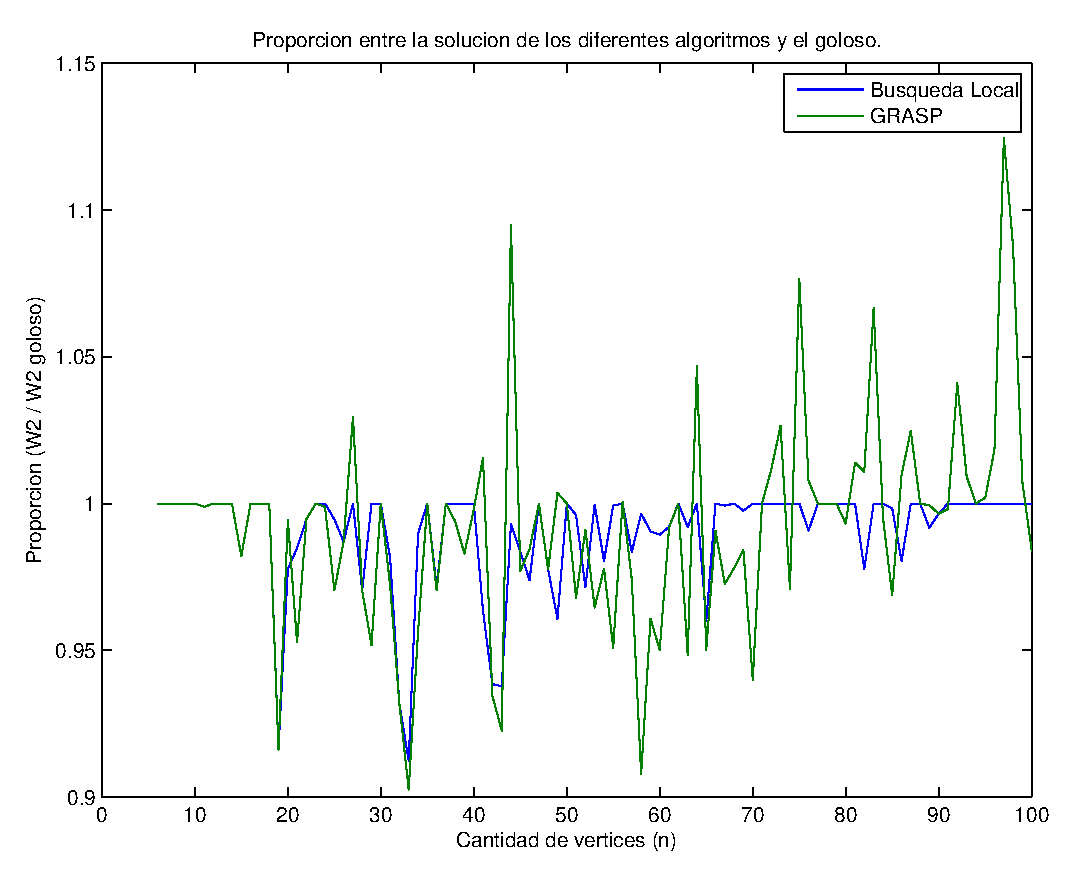
\includegraphics[width=\linewidth]{graficos/todos_calidad.eps}
    \caption{Soluciones en proporción con goloso }\label{fig:proporcion-goloso}
    \end{minipage}
  \end{center}
\end{figure}


El algoritmo de búsqueda local siempre da soluciones que son mejores o iguales a las que da el algoritmo goloso, ya que la proporción es siempre menor o igual a uno. Esto es lógico ya que nuestro algoritmo de búsqueda local toma como solución inicial la que da el goloso e intenta mejorarlas, lo cual no siempre logra, pero nunca empeora la solución inicial que se le da.

Además podemos ver que las soluciones que da el algoritmo GRASP son a veces mejores que las del algoritmo de búsqueda local pero a veces son peores. Esto es debido a que el algoritmo de GRASP hace búsqueda local sobre la solución inicial que le da nuestro algoritmo goloso aleatorio en cada iteración. Por lo tanto GRASP hace búsqueda local a partir de soluciones iniciales distintas a la del algoritmo de búsqueda local que toma como solución inicial la dada por nuestro algoritmo goloso que no es aleatorio. Entonces, tiene sentido que GRASP llegue a soluciones distintas al algoritmo de búsqueda local, las cuales a veces son mejores y a veces son peores.


\newpage

%%%%%%%%%%%%%%%%%%%%%%%%%%%%%%%%%%%%%%%%%%%%%%%%%%%%%%%%%%%%%%%%%%%%%%%%%%%%%%%
%% Conclusión                                                                %%
%%%%%%%%%%%%%%%%%%%%%%%%%%%%%%%%%%%%%%%%%%%%%%%%%%%%%%%%%%%%%%%%%%%%%%%%%%%%%%%

\section{Conclusión}
\label{sec:conclusion}
Para concluir, nos parece importante recalcar que ninguna heurística que planteamos es estrictamente mejor que todas las demás. Sin embargo, podemos asegurar que nuestro algoritmo de búsqueda local es siempre mejor o igual que nuestro algoritmo goloso, debido a por como está implementado. 

Otra punto que concluimos es que la diferencia entre nuestras 3 heurísticas, en general, no es grande. Creemos que esto se debe a que la vecindad propuesta no es muy bueno. Esto genera pocos cambios en la búsqueda local por lo que todas las heurísticas se parecen al algoritmo goloso. Una posible solución a esto es ampliar nuestra vecindad, generando las mismas operaciones pero en vez de a un nodo, de a $k$.

Esto tiene sentido, ya que una heurística es una técnica para resolver problemas donde la solución dada puede no ser óptima. Si pudiéramos dar la solución óptima	 en una cantidad de tiempo lo suficientemente chico, no tendría sentido hablar de heurísticas.

\newpage

%%%%%%%%%%%%%%%%%%%%%%%%%%%%%%%%%%%%%%%%%%%%%%%%%%%%%%%%%%%%%%%%%%%%%%%%%%%%%%%
%% Apéndices                                                                 %%
%%%%%%%%%%%%%%%%%%%%%%%%%%%%%%%%%%%%%%%%%%%%%%%%%%%%%%%%%%%%%%%%%%%%%%%%%%%%%%%

\begin{appendices}

\section{Algoritmo exacto}
\label{exacto-codigo}
\verbatiminput{./codigo-fuente/exacto.cpp}

\newpage

\section{Algoritmo de Dijkstra randomizado}
\label{dijkstra-codigo}

\verbatiminput{./codigo-fuente/dijkstra.cpp}

\newpage

\section{Algoritmo goloso}
\label{goloso-codigo}
\verbatiminput{./codigo-fuente/goloso.cpp}

\newpage

\section{Algoritmo búsqueda local}
\label{busqueda-local-codigo}
\verbatiminput{./codigo-fuente/busqueda.cpp}

\newpage

\section{Algoritmo tipo GRASP}
\label{grasp-codigo}
\verbatiminput{./codigo-fuente/grasp.cpp}


\end{appendices}

\end{document}